\documentclass{bachproef-tin}

\usepackage{hogent-thesis-titlepage} % Titelpagina conform aan HOGENT huisstijl
\usepackage{graphicx,caption,subfig,tabularx}
\usepackage{floatrow,enumitem,csquotes,pgfplots}

%%---------- Documenteigenschappen ---------------------------------------------


% De titel van het rapport/bachelorproef
\title{Een bedrijfsnetwerk beter beveiligen en beheren met behulp van Cisco Identity Services Engine}


\author{Joeri Verhavert}


\promotor{Olivier Rosseel}


\copromotor{Dean De Blieck}

\instelling{Axians - Fit IT}

% Academiejaar
\academiejaar{2019-2020}

% Examenperiode
%  - 1e semester = 1e examenperiode => 1
%  - 2e semester = 2e examenperiode => 2
%  - tweede zit  = 3e examenperiode => 3
\examenperiode{2}

%===============================================================================
% Inhoud document
%===============================================================================

\begin{document}



%---------- Titelblad ----------------------------------------------------------
\inserttitlepage

%---------- Samenvatting, voorwoord --------------------------------------------
%\usechapterimagefalse
%%=============================================================================
%% Voorwoord
%%=============================================================================

\chapter*{\IfLanguageName{dutch}{Woord vooraf}{Preface}}
\label{ch:voorwoord}

Met het schrijven van dit voorwoord leg ik het laatste hand aan mijn eindwerk. Het was me een periode waar ik heel veel heb bijgeleerd, vooral op business, maar ook op persoonlijk vlak.  Graag wil ik dan ook van deze gelegenheid gebruik maken om een aantal mensen te bedanken want zonder hen was dit nooit gelukt. 
\newline
\newline
In de eerste plaats wil ik mijn promotor, Olivier Rossel, bedanken. Dankzij de heer Rosseel kwam dit eindwerk in de goede banen terecht. Steeds toonde u mij de richting waar ik heen moest. Daarnaast nam u telkens opnieuw de tijd om mijn draft versies te overlopen en te controleren. Hiervoor een welgemeende danku!
\newline
\newline
Vervolgens wil ik graag mijn collega’s van het stagebedrijf Axians bedanken voor de fijne samenwerking en hulp die ik heb gekregen. Jullie hebben mij enorm gesteund en waren steeds bereid om mij te helpen. Bedankt!
\newline
\newline
Mevrouw Cousy, u nam in uw drukke agenda de tijd om dit eindwerk zorgvuldig na te lezen op spelling en op taal. Zonder u was deze bachelorproef een taal fiasco. Bedank!
\newline
\newline
Tot slot wil ik graag men ouders bedanken voor de vele inspanningen die zijn hebben geleverd in de afgelopen jaren. Jullie stonden steeds paraat na alle ups maar ook na alle downs. Dankuwel mama en papa!
\newline
\newline
Voor u ligt mijn eindwerk, een resultaat van wekenlang hard werken. Ik hoop dat het resultaat van mijn werk zichtbaar mag zijn en dat het u bekoort. 
\newline
\newline
Ik wens u veel leesplezier toe!
\newline
Joeri Verhavert





%%=============================================================================
%% Samenvatting
%%=============================================================================

% TODO: De "abstract" of samenvatting is een kernachtige (~ 1 blz. voor een
% thesis) synthese van het document.
%
% Deze aspecten moeten zeker aan bod komen:
% - Context: waarom is dit werk belangrijk?
% - Nood: waarom moest dit onderzocht worden?
% - Taak: wat heb je precies gedaan?
% - Object: wat staat in dit document geschreven?
% - Resultaat: wat was het resultaat?
% - Conclusie: wat is/zijn de belangrijkste conclusie(s)?
% - Perspectief: blijven er nog vragen open die in de toekomst nog kunnen
%    onderzocht worden? Wat is een mogelijk vervolg voor jouw onderzoek?
%
% LET OP! Een samenvatting is GEEN voorwoord!

%%---------- Nederlandse samenvatting -----------------------------------------
%
% TODO: Als je je bachelorproef in het Engels schrijft, moet je eerst een
% Nederlandse samenvatting invoegen. Haal daarvoor onderstaande code uit
% commentaar.
% Wie zijn bachelorproef in het Nederlands schrijft, kan dit negeren, de inhoud
% wordt niet in het document ingevoegd.

\IfLanguageName{english}{%
\selectlanguage{dutch}
\chapter*{Samenvatting}

\selectlanguage{english}
}{}

%%---------- Samenvatting -----------------------------------------------------
% De samenvatting in de hoofdtaal van het document

\chapter*{\IfLanguageName{dutch}{Samenvatting}{Abstract}}

Dit onderzoek kan dienen om bedrijfsnetwerken beter te beheren en beveiligen tegen interne of externe gevaren met behulp van Cisco Identity Services Engine. Dit omdat bedrijfsnetwerken steeds meer nood hebben aan een network access control product die netwerken beter kunnen beheren en beveiligen. Dit onderzoek focust zich voornamelijk op implementatie en evaluatie van Cisco Identity Services Engine met use cases 'Port-based access control', 'Policy-based access control' en 'Tread-Centric access control'. 
\newline
\newline
Daarnaast worden de resultaten van de enquête tijdens dit onderzoek geanalyseerd die op het einde mee verwerkt zijn met de evaluatie van Cisco Identity Services Engine en zijn use cases. In de literatuurstudie zijn twee andere network access control producten mee verwerkt om aan te tonen dat integratie van deze network access control producten ook mogelijk zijn om een netwerk robuster te maken. Bij de analyses wordt een netwerk geanalyseerd voor integratie van de use cases en eens na de integratie van de use cases. Uit deze twee vergelijkingen werd een evaluatie opgesteld. In dit geschrift vindt u een inleiding tot het onderwerp dat verwerkt is in de literatuurstudie. Daarnaast vindt u de resultaten van de uitgevoerde testen en van de enquête in Hoofdstuk \ref{ch:Resultaten}. 
\newline
\newline
Uit dit onderzoek blijkt dat integratie van Cisco Identity Services Engine de vruchten plukt op beheersbaarheid en beveiliging, dit wordt ook bevestigd in de enquête resultaten. Vervolgens komt uit de enquête naar voor dat 'Identity-based access control' voor vakspecialisten de belangrijkste use case is binnen het Cisco Identity Services Engine product. Toekomstig onderzoek kan over 'Identity-based access control' uitgevoerd worden dat de voordelen van deze use case naar boven brengt.


%---------- Inhoudstafel -------------------------------------------------------
\pagestyle{empty} % Geen hoofding
\tableofcontents  % Voeg de inhoudstafel toe
\cleardoublepage  % Zorg dat volgende hoofstuk op een oneven pagina begint
\pagestyle{fancy} % Zet hoofding opnieuw aan

%---------- Lijst figuren, afkortingen, ... ------------------------------------


\listoffigures
\listoftables
%%=============================================================================
%% Inleiding
%%=============================================================================

\chapter{\IfLanguageName{dutch}{Inleiding}{Introduction}}
\label{ch:inleiding}

\begin{displayquote}
	“It takes 20 years to build a reputation and few minutes of cyber-incident to ruin it.” – Stephane Nappo
\end{displayquote}

De quote van Stephane Nappo, Global Chief Information Security Officer, expliceert met zijn quote het belang van cybersecurity in een notendop. Cybersecurity is namelijk één van de meest besproken technologische onderwerpen die centraal staan in bedrijven die 'oorlog' voeren met cyber criminelen. Information and Communications Technology wordt de dag vandaag alsmaar grootschaliger toegepast en zal in de nabije toekomst zeker niet verminderen. Door de grote uitbreiding in Information and Communications Technology stijgt de kans op cyber aanvallen evenredig mee. Persoonlijke gegevens of resources kunnen door de stijging in cyber aanvallen sneller gestolen worden dan 20 jaar geleden. Een oplossing was dus hoognodig, waardoor het cybersecurity begrip ontstond. 
\newline
\newline
Daarbij moeten organisaties sterk investeren om de aanvalspogingen drastisch te doen verminderen om zo de cyber criminelen een stapje voor te zijn. Nieuwe principes zoals 'Internet of Things' en 'Bring Your Own Device' maken bedrijven het er niet gemakkelijker op. Vanuit dit probleem kwam Axians met de vraag voor dit onderzoek, waarbij het gebruik van Cisco Identity Services Engine in samen werking met 'Policy-based access control', 'Port-based access control' en Thread-Centric access control centraal staat. Cisco Identity Services Engine is een network access control product dat de handhaving van beveiligings- en toegangsbeleid mogelijk maakt voor eind apparaten die zijn aangesloten op het netwerk apparatuur van het bedrijf. Het doel is om identiteitsbeheer en om het veiligsbeheer op verschillende eind apparaten en applicaties te vereenvoudigen.
\newline
\newline
Hieruit is de onderzoeksvraag '\textit{Een bedrijfsnetwerk beter beveiligen en beheren met behulp van Cisco Identity Services Engine}' ontstaan, waarbij volgende doelstellingen mee bedacht zijn: 

\begin{itemize}
	\item Implementatie van Cisco Identity Services Engine in een netwerk.
	\item Integratie van 'Port-based access control met Cisco Identity Services Engine in een netwerk.
	\item Integratie van 'Policy-based access control met Cisco Identity Services Engine in een netwerk.
	\item Integratie van 'Thread-Centric access control met Cisco Identity Services Engine in een netwerk.
	\item Evaluatie van Cisco Identity Services Engine in een netwerk.
\end{itemize}

De samenleving en de Information and Communications technologieën zullen steeds verder evolueren waardoor ondernemingen in staat moeten om cybersecurity steeds te blijven opvolgen. Men zal constant moeten bijleren om de strijd tegen cyberaanvallen te blijven winnen. De opvolging wordt er zeker en vast niet gemakkelijker op, waardoor dit efficiënter verloopt als men in team werkt. Cybersecurity vereist dus een samenwerking om de resources en gegevens te beschermen.

\section{\IfLanguageName{dutch}{Probleemstelling}{Problem Statement}}
\label{sec:probleemstelling}
Aangezien Information and Communications Technology zou centraal staat in de 21ste eeuw kan iedereen in aanraking komen met cyber aanvallen. Denk maar aan de talrijke pogingen die cyber criminelen via Facebook, Twitter, E-mail, enz. proberen om accounts, geld, informatie te bemachtigen bij deze slachtoffers. Veel van deze gevallen gebeuren op individueel vlak, maar bedrijven hebben evenveel risco's om besloten te worden. Men kan verschillende methodes bedenken hoe organisaties het slachtoffer kan zijn van cyberaanvallen. Maar dit onderzoek focust zich pricipes zoals 'Internet of Things' en 'Bring Your Own Device'.
\newline
\newline
Hierdoor wordt het doelgroep van dit onderzoek beperkt met oog op de eind apparaten die het netwerk steeds verlaten en opnieuw binnen komen, specifiek zal het onderzoek zich richten op de eind apparaten van de werknemers van Axians die gebruiken maken van het netwerk. Aangezien deze eind apparaten het netwerk flink kunnen toetakelen.


\section{\IfLanguageName{dutch}{Onderzoeksvraag}{Research question}}
\label{sec:onderzoeksvraag}
Een veiliger en beter beheerbaarder netwerk is wat men wil bereiken door het gebruik van een network access control product en use cases zoals :'\textit{Port-based access control, Policy-based access control}' en '\textit{Thread-Centric access control}'. Dit network access control product is Cisco Identity Services Engine.

De hoofdstuk onderzoeksvraag in deze bachelorproef is: 
\begin{displayquote}
	Hoe kunnen we een evoluerend bedrijfsnetwerk beter beveiligen door het gebruik van Cisco ISE?
\newline
\newline
\end{displayquote}
Verder zal deze bachelorproef zich verdiepen in het gebruik van Cisco's Identity Services Engine use cases. 
\begin{displayquote}
	Welke invloed heeft de integratie van \textit{Port-based access control} in een netwerk?  
\newline
\newline
	Wat is meerwaarde van de integratie van \textit{Policy-based access control} in een netwerk?  
\newline
\newline
	Kan het netwerk wel degelijk beschermt worden tegen verder uitbreiding van Malware door integratie van \textit{Thread-Centric access control} in een netwerk?  
\end{displayquote}

\section{\IfLanguageName{dutch}{Onderzoeksdoelstelling}{Research objective}}
\label{sec:onderzoeksdoelstelling}

%Wat is het beoogde resultaat van je bachelorproef? Wat zijn de criteria voor succes? Beschrijf die zo concreet mogelijk. Gaat het bv. om een proof-of-concept, een prototype, een verslag met aanbevelingen, een vergelijkende studie, enz.
Door middel van Cisco Identity Services Engine network access control product zal dit onderzoek inzicht bieden op het beveiligen en beter beheren van netwerken tegen interne of externe gevaren. Vervolgens moeten de resultaten van de enquête een eenduidig antwoord bieden die in lijn liggen met de resultaten van de uitgevoerde testen, enkel dan is dit deelonderzoek geslaagd. Door dit onderzoek wil men dat ondernemingen stappen zetten in de juiste richting tegen de strijd met cyber criminelen. Zo kan informatie, geld en andere resource in bedrijven gewaarborgd blijven. Wanneer bedrijven de waarde van een network access control inzien, dan is dit onderzoek volledig geslaagd.

\section{\IfLanguageName{dutch}{Opzet van deze bachelorproef}{Structure of this bachelor thesis}}
\label{sec:opzet-bachelorproef}

% Het is gebruikelijk aan het einde van de inleiding een overzicht te
% geven van de opbouw van de rest van de tekst. Deze sectie bevat al een aanzet
% die je kan aanvullen/aanpassen in functie van je eigen tekst.

De rest van deze bachelorproef is als volgt opgebouwd:

In Hoofdstuk~\ref{ch:stand-van-zaken} wordt een overzicht gegeven van de stand van zaken binnen het onderzoeksdomein, op basis van een literatuurstudie.

In Hoofdstuk~\ref{ch:methodologie} wordt de methodologie toegelicht en worden de gebruikte onderzoekstechnieken besproken om een antwoord te kunnen formuleren op de onderzoeksvragen.

In Hoofdstuk~\ref{ch:Proof of concept} wordt een overzicht gegeven van de omgeving en de gebruikte tools voor implemenatie van Cisco Identity Services Engine. 

In Hoofdstuk~\ref{ch:Resultaten} worden de resultaten van de uitgevoerde testen en van de enquête toegelicht.

In Hoofdstuk~\ref{ch:conclusie}, tenslotte, wordt de conclusie gegeven en een antwoord geformuleerd op de onderzoeksvragen. Daarbij wordt ook een aanzet gegeven voor toekomstig onderzoek binnen dit domein.
 \chapter{\IfLanguageName{dutch}{Literatuurstudie}{State of the art}}
\label{ch:stand-van-zaken}

% Tip: Begin elk hoofdstuk met een paragraaf inleiding die beschrijft hoe
% dit hoofdstuk past binnen het geheel van de bachelorproef. Geef in het
% bijzonder aan wat de link is met het vorige en volgende hoofdstuk.

% Pas na deze inleidende paragraaf komt de eerste sectiehoofding.
%
%Dit hoofdstuk bevat je literatuurstudie. De inhoud gaat verder op de inleiding, maar zal het onderwerp van de bachelorproef *diepgaand* uitspitten. De bedoeling is dat de lezer na lezing van dit hoofdstuk helemaal op de %hoogte is van de huidige stand van zaken (state-of-the-art) in het onderzoeksdomein. Iemand die niet vertrouwd is met het onderwerp, weet nu voldoende om de rest van het verhaal te kunnen volgen, zonder dat die er nog andere informatie moet over opzoeken \autocite{Pollefliet2011}.

%Je verwijst bij elke bewering die je doet, vakterm die je introduceert, enz. naar je bronnen. In \LaTeX{} kan dat met het commando \tt{$\backslash${textcite\{\}}} of \texttt{$\backslash${autocite\{\}}}. Als argument van het commando geef je de ``sleutel'' van een ``record'' in een bibliografische databank in het Bib\LaTeX{}-formaat (een tekstbestand). Als je expliciet naar de auteur verwijst in de zin, gebruik je \texttt{$\backslash${}textcite\{\}}.
%Soms wil je de auteur niet expliciet vernoemen, dan gebruik je \texttt{$\backslash${}autocite\{\}}. In de volgende paragraaf een voorbeeld van elk.

Deze literatuurstudie richt zich op cybersecurity in zijn geheel. Daarnaast zijn er een aantal belangrijke begrippen verder uitgeschreven die tijdens deze bachelorproef aan bod komen. Op deze manier is er een systematische studie uitgevoerd die een omliggende context creëert omtrent network access control technologieën zoals Cisco Identity Services Engine en dergelijke andere producten. 
\newline
\newline
Verder is er een studie uitgevoerd over een aantal network access control producten zoals Portnox, Aruba ClearPass Policy Manager en de belangrijkste van dit onderzoek, namelijk Cisco Identity Services Engine. Het onderwerp omtrent Cisco Identity Services Engine werd in samenspraakt met Axians besloten. Voor beide partijen leek Cisco Identity Services Engine het interessantst om een onderzoek over uit te voeren. Cisco Identity Services Engine wordt hierbij ook toegepast in de omgeving van Axians. Vervolgens wordt dit onderzoek ingeleid met een kort woordje uitleg over het network access control begrip. 
\newline
\newline
Dit wordt gevolgd met een toelichting van de drie network access control producten. Nadien wordt een extra woordje uitleg gegeven over reeds bestaande onderzoeken die antwoorden bieden op gelijkaardige onderzoeksvragen zoals deze bachelorproef.
\newline
\newline
Ten slot wordt deze literatuurstudie afgesloten met een kleine vergelijking en een conclusie over deze technologieën. 

\newpage

\section{Algemene cybersecurity}
Als er even wordt teruggekeken naar het verleden, dan was er 40 jaar geleden nog geen sprake van cybersecurity. Iedereen weet natuurlijk dat de technologie van toen nog niet zo gevorderd was zoals de dag van vandaag. De samenleving toen bestond nog niet uit miljoenen apparaten die met het internet waren verbonden, laat staan dat het internet in die mate zelf bestond. Dus waarom zou er dan ooit sprake geweest zijn van cybersecurity?
\newline
\newline 
In deze nieuwe samenleving wordt Information and Communications Technology (kortweg ICT) grootschalig toegepast. Deze ontwikkeling bood de samenleving heel wat economische groei, gevolgd door heel wat nieuwe online gevaren. Gehackt worden, is de dag van vandaag één van die nieuwe gevaren waarbij men zeker moet bij stil staan. Niemand wilt natuurlijk dat onze persoonlijke gegevens op straat komen te liggen. Uit deze nieuwe gevaren en kwetsbaarheden is cybersecurity ontstaan. Maar wat is cybersecurity? Waarom is het zo belangrijk? Wat komt erbij kijken? Hoe stellen we cybersecurity op?
\newline
\newline
\cite{AlexTarter2017} schreef een prachtig artikel over het belang van cybersecurity. Hij probeerde op zijn manier de nadruk te leggen op de belangrijkste concepten van cybersecurity. Hiervoor verwees hij naar de nieuwe technologieën die cyber criminelen met open armen ontvangen. Het is vaak zo dat nieuwe technologieën gepaard gaan met vele kwetsbaarheden. Volgens \cite{AlexTarter2017}, zijn deze kwetsbaarheden de ideale omgevingen voor cyber criminelen om informatie, geld, of andere zaken te ontnemen. Hierdoor legt hij de nadruk op deze gevaren door de verschillende hacking technieken uit te leggen en hoe men zich hiertegen kan beschermen. 

\section{Wat is cybersecurity?}
Cybersecurity omvat het beschermen van netwerken, computers, mobiele apparatuur, elektronische systemen en servers tegen schadelijke online aanvallen. Dit is ook wel bekend als de beveiliging van de elektronische gegevens. Cybersecurity heeft betrekking op alle maatregelen die worden genomen om netwerken, programma’s en eind apparaten te verdedigen tegen digitale criminaliteit. Organisaties, overheden en gezinnen worden beschermd tegen deze duistere pogingen om persoonlijke gegevens te bemachtigen.
\newline
\newline 
Het is van groot belang dat er preventieve, detective en correctieve maatregelen zijn, onder de vorm van procedures, policies of processen. Deze maatregelen worden opgesteld om de integriteit en beschikbaarheid van informatie binnen organisaties, overheden en zelfs gezinnen te garanderen. Door de implementatie van deze maatregelen kan er op een analytische graad, het gewenste niveau van beveiliging bepaald worden. Hieruit is een security model ontwikkeld waarbij specialisten stil staan bij de verschillende onderdelen van Information Technologie Security (ook gekend als IT Security). Dit security model noemt men het CIA Triad model. 

\subsection{CIA Traid}
CIA Triad is een Engelstalig begrip waarmee de principes van informatiebeveiliging worden aangeduid aan de hand van een driehoek. CIA Triad bevat drie verschillende voorwaarden voor een goede informatiebeveiliging. Deze voorwaarden komen ook terug in de benaming, CIA. Confidentiality, Integrity en Availability is de onafgekorte versie van de 'CIA' afkorting. Vertaald naar het Nederlands betekent dit: Beschikbaarheid, Integriteit en Vertrouwelijkheid. Hierbij zijn de pricipes van CIA Triad terug te vinden in de figuur \ref{fig:CIATraid}. De Nederlandse benaming voor CIA Triad noemt men het BIV-classificatie - of het BIV-indelings model. Belangrijk om te weten is dat wanneer men spreekt over security, de drie elementen of principes van het BIV-classificatie model tot één van de meest belangrijkste componenten van security behoren. 
\newline
\newline 
Verder moet er zeker vermeld worden dat sinds de opkomst of vooruitgang van technologieën zoals Big Data en Internet of Things, nieuwe uitdaging moeten worden opgesteld voor het BIV-classificatie model en voor cybersecurity in het algemeen.
\newline
\newline  
Eén van de uitdagingen van CIA Triad model met combinatie van Internet of Things, is de beveiliging ervan. Tot op de dag van vandaag ontdekt men verschillende mogelijkheden die de beveiliging van deze systemen doorbreekt. Patches of updates worden dikwijls niet snel vrijgegeven. Als gevolg leidt dit tot een grote bezorgdheid, aangezien een groter gebruik van deze systemen binnen een netwerk, onrechtstreeks navigeert naar persoonlijke gegevens.
\newline
\newline 
Het artikel van \cite{Samonas2014} mag zeker bekeken worden. Hij herbekeek het CIA Triad model en gaf een uitgebreide beschrijving over het CIA Triad model en zijn drie pilaren. In de onderstaande alinea’s vindt u een korte samenvatting over deze drie pilaren die \cite{Samonas2014} beschreef in zijn paper.

\subsubitem{\bf Vertrouwelijkheid}
\newline
Het vertrouwelijkheids principe (Confidentiality) van CIA-Triad zorgt er voor dat alleen die personen voor wie de informatie of data bedoeld is, toegang krijgen tot deze data. Als volgt kan er gewaarborgd worden dat enkel de geautoriseerde personen toegang krijgen tot deze data. Hierdoor kan deze informatie niet verder gepubliceerd worden, omdat men dit vaak gerefereert naar de privacybescherming. 
\subsubitem{\bf Integriteit}
\newline
Verder is er het integriteits principe (Integrity) binnen het CIA Triad model. Dit verwijst naar de data, die correct en volledig moet zijn. Dit principe moet er voor zorgen dat personen die toegang vragen tot bepaalde data, de volledige data, en niet gemanipuleerde data ontvangen. 
\newpage
\subsubitem{\bf Beschikbaarheid}
\newline
Als laatste is er het beschikbaarheids principe (Availability). Dit principe beschrijft de mate waarin bij voorkeur geautoriseerde personen, programmatuur of apparatuur gebruik kunnen maken van de gegevens. Dit kan al dan niet gereguleerd gebeuren door (geautomatiseerde) procedures en/of technische maatregelen. 

\begin{figure}[H]
	\centering
	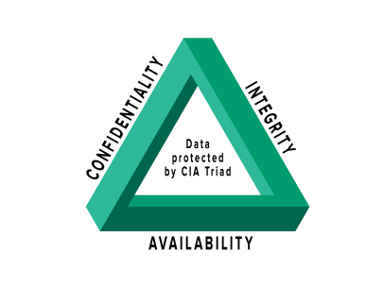
\includegraphics[width=0.5\textwidth]{CIATraid.png}
	\caption{Principes van het CIA Triad model (\cite{PrincipesCIA})}
	\label{fig:CIATraid}
\end{figure}

\subsection{Triple A }
Triple A of kortweg AAA, is de afkorting voor Authentication, Authorization en Accounting. Triple A definieert een architectuur die gebruikers authenticeert, autoriseert en de activiteiten logt. Met andere woorden wordt AAA gebruikt om de toegang te verschaffen naar elektronische systemen of netwerken.
\newline
\newline
Vaak spreekt men over een “open” netwerkarchitectuur wanneer AAA niet wordt toegepast binnen een infrastructuur. In deze “open” netwerkarchitectuur heeft iedereen toegang tot alle systemen, met als gevolg dat éénder wie alles kan uitvoeren zonder enige tracking.
\newline
\newline
In onderstaande alinea’s is er een zorgvuldige beschrijving van de drie A’s terug te vinden.
\subsubitem{\bf Authenticatie}
\newline
Tn dit proces wordt de identiteit van de persoon die een bepaalde dienst of service wenst te gebruiken nagegaan. Tijdens dit proces worden gegevens uitgewisseld om de identiteit van de gebruiker te kunnen verifiëren. Voorbeelden hiervan zijn: combinatie van gebruikersnaam en wachtwoord, het gebruik van een vingerprint scanning om in te loggen in bepaalde systemen, enz.
\newpage
\subsubitem{\bf Autorisatie}
\newline 
Autorisatie is het proces waarbij de rechten van iemand gecontroleerd wordt of hij beschikt over de juiste rechten om bepaalde diensten en/of services te contacteren. Met andere woorden wordt de vastgestelde identiteit gebruikt om te bepalen welke rechten de gebruiker heeft. Dikwijls wordt tijdens het vaststellen van deze rechten andere gegevens vastgelegd. Voorbeelden hiervan zijn: toewijziging van een IP adres, tijdslimiteringen, enz.

\subsubitem{\bf Accounting}
\newline
Accounting is het proces waarbij de gebruikte services of diensten van de vastgestelde gebruiker wordt bijgehouden. Deze informatie kan gebruikt worden voor doeleinden zoals management, facturatie, enz. Typische informatie die heel vaak wordt bijgehouden zijn, de vastgestelde identiteit van de gebruiker, het type dienst dat gebruikt werd of bepaalde tijdstippen wanneer men gebruik maakte van de verschillende diensten of services. 

\section{Bring Your Own Device}
BYOD staat voor “Bring Your Own Device”, ook wel "Bring Your Own Technology" genoemd. Dit is een concept waarbij iedereen binnen de organisatie zijn eigen apparatuur meebrengt naar het werk. Hierbij wordt veelal gerefereerd naar mobiele apparatuur, zoals smartphones, tablets, laptops, maar ook complete desktopcomputers die zakelijk gebruikt worden behoren ook tot deze trend. Deze talrijke systemen maken in vele situaties gebruik van de verschillende bedrijfsmiddelen zoals e-mail, file servers, databases en talrijke andere bedrijfsmiddelen.
\newline
\newline
De paper van \cite{Zakiah2017} meldt dat de opkomst van Bring Your Own Device behoorlijke opportuniteiten meebrengt voor hackers. Deze hackers vinden steeds meer nieuwe kwetsbaarheden die gevoelige data of informatie van werknemers of studenten uitbuit. Het zich bewust laten maken van deze veeltalige risico's aan de personen, is volgens \cite{Zakiah2017} de eerste stap tegen de opmars van online aanvallen op de 'Bring Your Own Technology' systemen.
\newline
\newline
Een uitgebreid beleid is dus een goede stap in de juiste richting om het bedrijfsnetwerk veiliger te maken, maar vaak is dit niet voldoende om het netwerk te bestendigen tegen cyberaanvallen. De implementatie van een network access control product kan hiervoor een oplossing bieden volgens \cite{Zakiah2017}.

\section{Internet of Things}
Als men aan Internet of Things (ofwel IoT) denkt, dan denkt men waarschijnlijk aan apparaten zoals smartphones of laptops, maar Internet of Things omvat veel meer dan dat. Het bestaat uit fysieke voorwerpen zoals huishoudelijke apparaten, wearables, kopieerapparaten, koelkasten of om het even welk fysiek apparaat dat met het internet verbonden is.
\newline
\newline 
Deze internetgebruikers worden de zogenaamde embedded systems genoemd. Zij kunnen communiceren met personen maar ook met andere embedded systems. Vaak is de communicatie simpel en eenvoudig, waardoor de embedded systems (ofwel Internet of Things apparaten) een kwetsbaarheid vormen in het bedrijfsnetwerk.
\newline
\newline
Wanneer er de paper van \cite{Salim2016} wordt bijgehaald, dan kan men afleiden dat Internet of Things infrastructuren en services, grote security uitdagingen ondervindt in elke omgeving. \cite{Salim2016} dicteerde het ‘Internet of Things security framework for smart infrastructures’ artikel die een duidelijker beeld schept over de integratie van smart homes of smart buildings met Internet of Things. Daarom ontworp \cite{Salim2016} een ‘threat model’ die een security methodologie voorstelt tegen cyber aanvallen. 
\newline
\newline
Om die reden is zoals bij Bring Your Own Device een uitgebreid beleid niet voldoende, maar kan een implementatie van een network access control product binnenin een bedrijfsomgeving de vruchten plukken op vlak van cybersecurity.  

\section{Network access control}
Nu reeds termen zoals Bring Your Own Device en Internet of Things uitgeklaard zijn, zal de betekenis en het belang van network access control technologieën verder uitgelegd worden.
\newline
\newline 
Een network access control is een type cyber security technologie waarmee ondernemingen beleidsregels kunnen implementeren en definiëren die de toegang van eind apparaten tot een bedrijfsnetwerk kunnen regelen. Tegelijkertijd biedt een network access control product een zichtbaarheid van apparaten die toegang proberen te krijgen met het netwerk, zodanig dat de veiligheid van het netwerk beter in kaart kan gebracht worden. Vervolgens wordt het belang van de implementatie van een network access control product in een netwerk toegelicht.
\newline
\newline 
Werknemers die met hun internet verbonden apparaten regelmatig inloggen op andere netwerken, maken de infrastructuur van hun eigen onderneming kwetsbaarder. Deze reizende systemen hebben een grotere kans om geïnfecteerd te worden met malware, dan apparatuur dat zich steeds binnen de muren van de onderneming bevindt. Een network access control product kan dus een oplossing bieden wanneer geïnfecteerde systemen toegang proberen te verschaffen in het netwerk. Dit is mogelijk dankzij Cisco's nieuwe 2.2 feature, namelijk Thread-centric access control. 
\newline
\newline 
De definitie en het belang van een network access control product werd alvast uitgelegd. In onderstaande alinea’s wordt er een woordje uitleg gegeven over drie nauwe, bijeenliggende network access control technologieën. Cisco Identity Services Engine werd gekozen in samenspraak met Axians. ‘Aruba ClearPass Policy Manager’ en ‘Portnox’ zijn network access control technologieën die willekeurig gekozen zijn op het internet. Vervolgens is er op het einde een kleine conclusie geschreven die dieper ingaat waarom er uiteindelijk gekozen werd voor Cisco Identity Services Engine en niet voor de overige network access control technologieën.

\subsection{Network access control technologieën}
\subsubsection{\bf Aruba ClearPass Policy Manager}
De Aruba ClearPass Policy Manager (\cite{ArubaCPPM})is een platform dat zorgt voor een veilige toegangscontrole tot een netwerk. Dit network access control (NAC) product is ontwikkeld omwille van de evolutie van smartphones, Bring Your Own Device en talrijke andere draadloze toepassingen. 
\newline
\newline
Netwerksecurity wordt de dag van vandaag steeds belangrijker en cyberaanvallen worden steeds geavanceerder. Met als gevolg moet privacygevoelige data binnen het netwerk blijven en mag enkel toegankelijk zijn voor geautoriseerde gebruikers. Aruba ClearPass Policy Manager biedt hiervoor een oplossing door gebruik te maken van een aantal uitgebreide zaken zoals o.a. , uitgebreide rapportages, ingebouwde AAA services zoals Radius, TACACS+, Kerberos, 802.1X, web radius authenticatie en dergelijke meer. In figuur \ref{fig:ArubaClearPass} zijn een aantal modules weergegeven binnen het Aruba ClearPass Policy Manager platform. 

\begin{figure}[H]
	\centering
	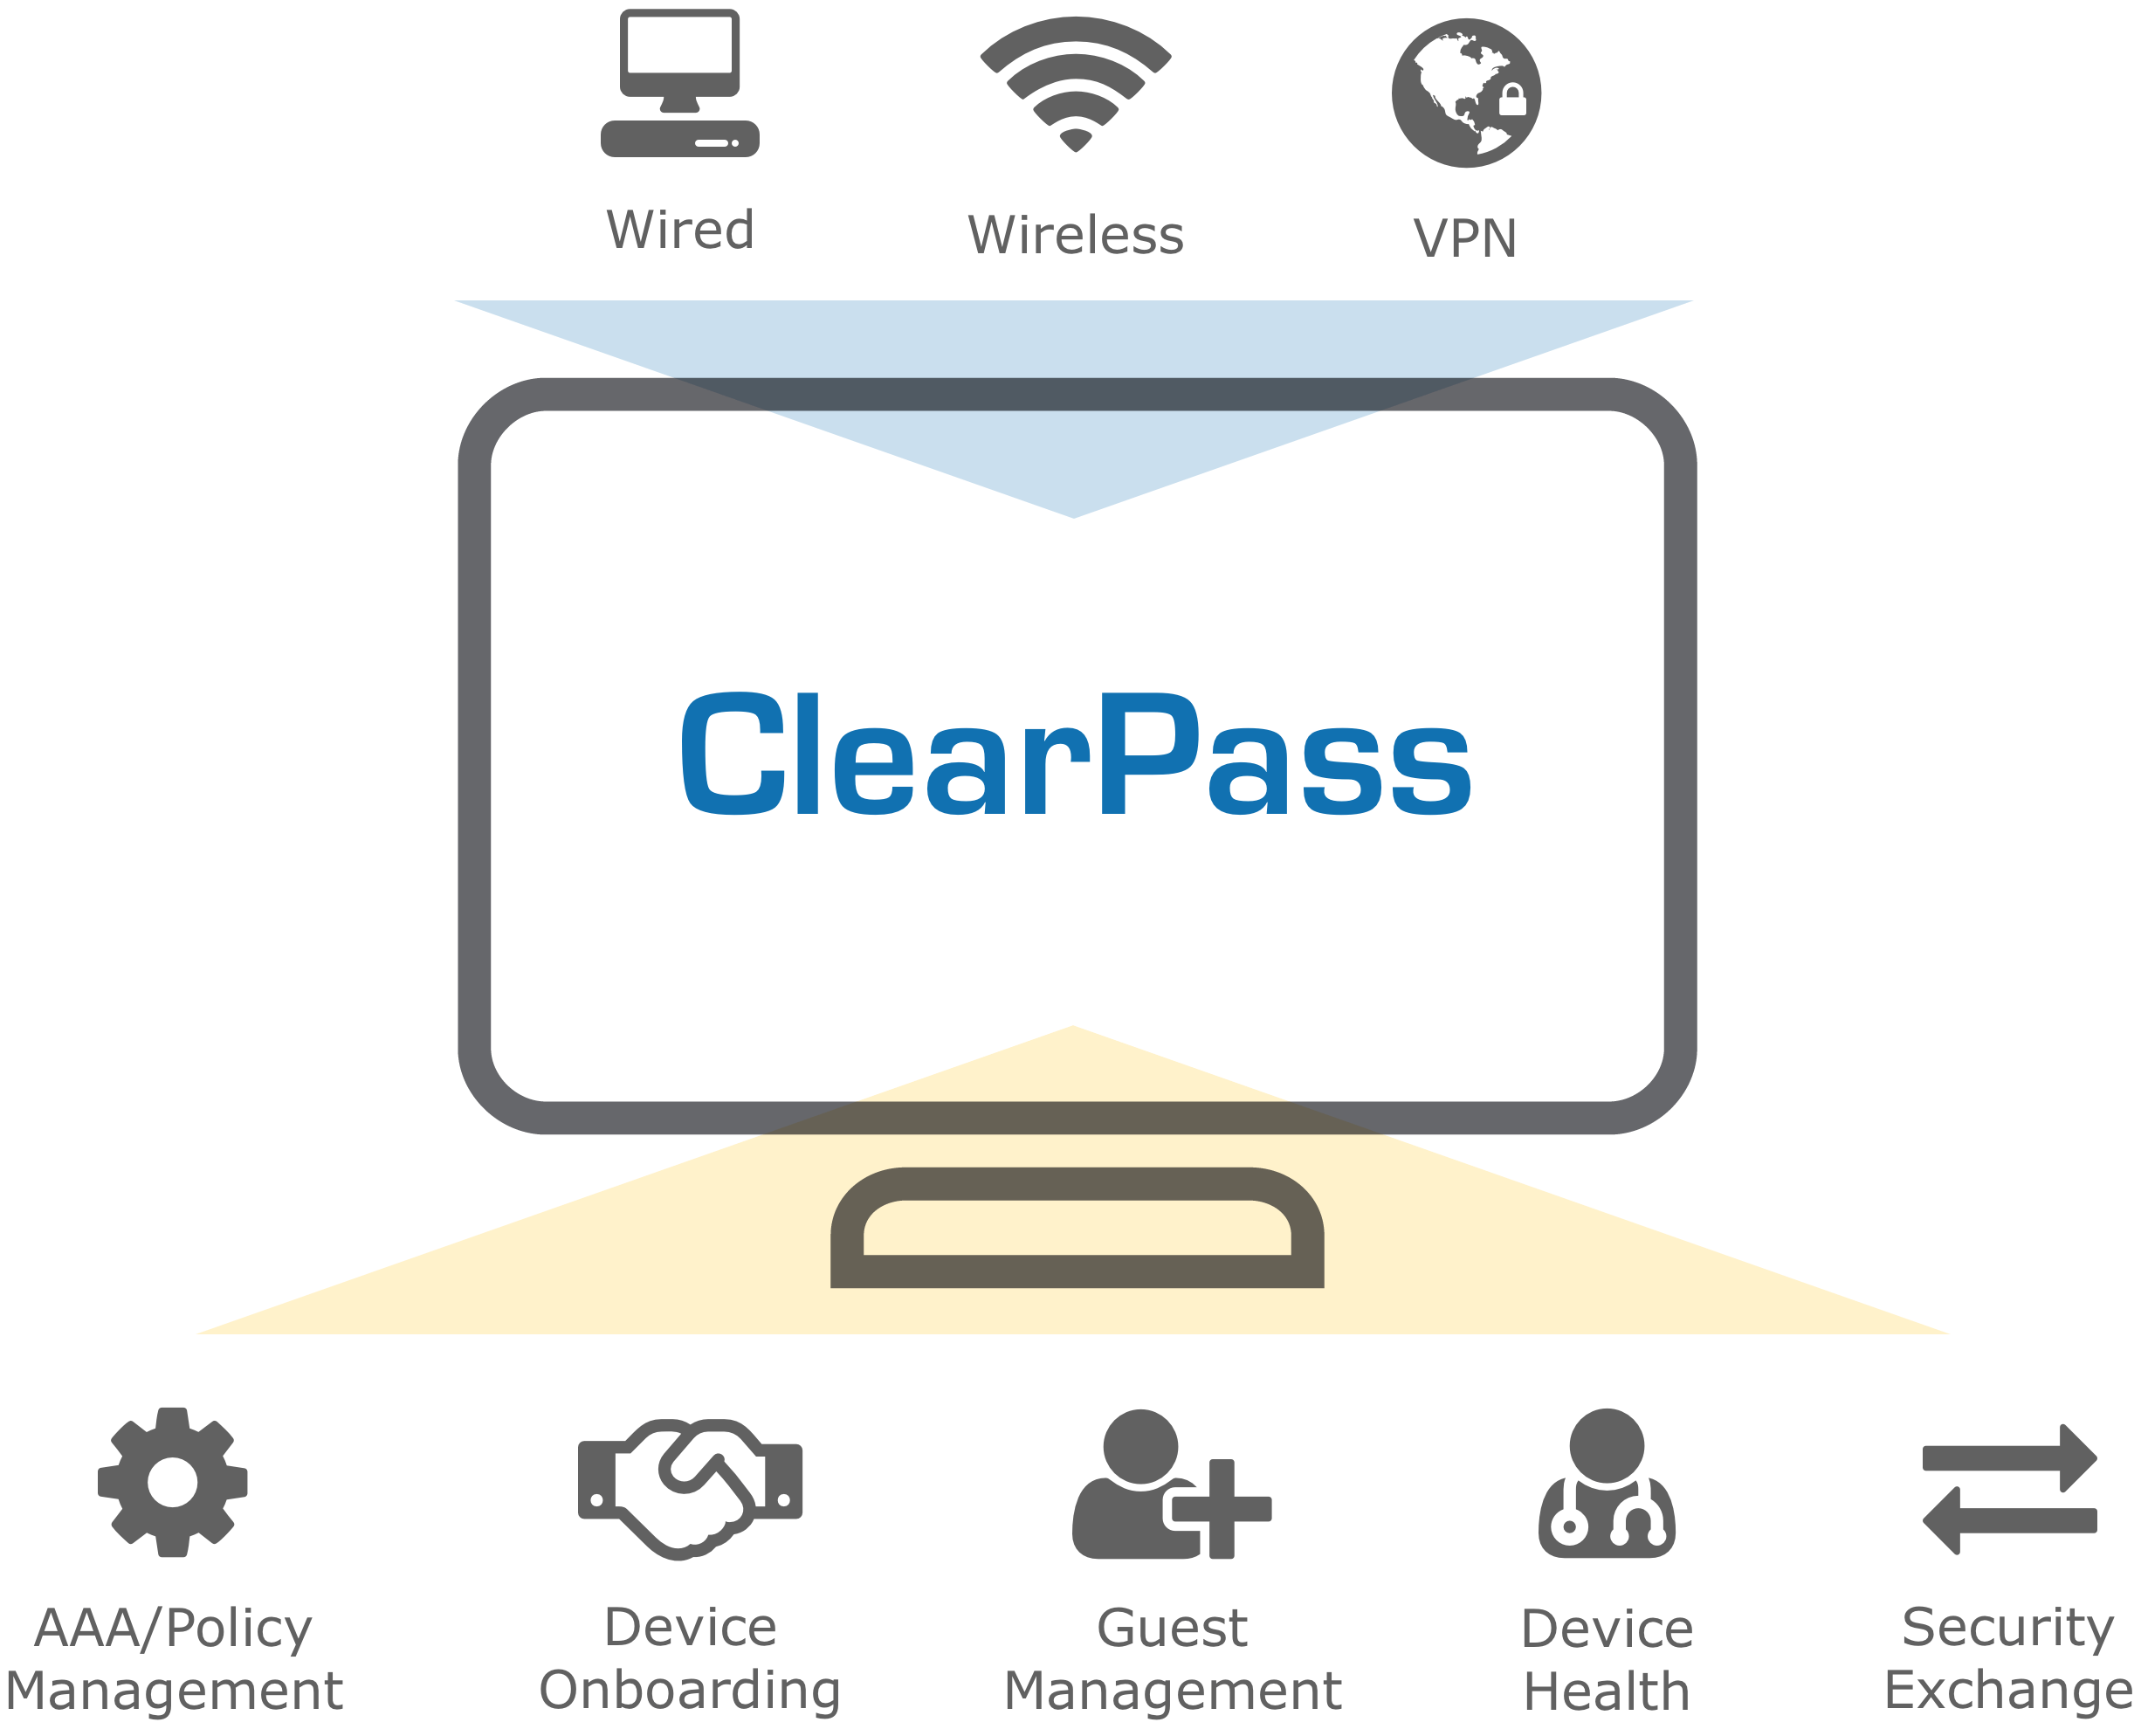
\includegraphics[width=0.5\textwidth]{Clearpass_authentication.png}
	\caption{Modules binnen het Aruba CPM platform (\cite{ACPMModule})}
	\label{fig:ArubaClearPass}
\end{figure}

\subsubsection{\bf Portnox}
Vervolgens is er het network access control technologie, genaamd \cite{Portnox}. Portnox is een network access control oplossing die vanuit de cloud wordt geleverd. Dit zijnde als ‘cloud as a service’. Desniettegenstaande dat dit ook mogelijk is om als on-premise gecentraliseerde software te gebruiken. Dit uit zich agentlesss op elk eind apparaat binnen in het bedrijfsterrein, of het nu Internet of Things is, Bring Your Own Device of door een ander bedrijf beheerd apparaat. In figuur \ref{fig:Portnox} is het logo van Portnox terug te vinden.
\newline
\newline
De veelzijdigheid van Portnox, maakt implementaties in de verschillende sectoren mogelijk. Dit zorgt er voor dat Portnox ook in het lijstje bevindt als competente kandidaten van network access control technologieën. Natuurlijk is het aanbod van competente network access control technologieën veel groter, maar deze literatuurstudie werd beperkt tot deze drie technologieën. 

\begin{figure}[H]
	\centering
	
\includegraphics[width=0.5\textwidth]{Portnox.png}
	\caption{Logo Portnox (\cite{PortnoxLogo})}
	\label{fig:Portnox}
\end{figure}

\subsubsection{\bf Cisco Identity Services Engine}
Cisco Identity Services Engine(\cite{ISE}) is een netwerkpunt waar alle methodes en identiteiten voor netwerktoegang worden geverifieerd aan de hand van gedefinieerde regelsets en authenticatiebronnen. Op basis van deze gedefinieerde regelsets en authenticatiebronnen kan Identity Service Engine toegangsrechten bieden tot bepaalde services. Factoren zoals: Active Directory groep, fysieke locatie van de gebruiker, OS-versie, enz. bepalen het type service dat gebruikt kan worden. Het doel is dus met andere woorden het vereenvoudigen van de identiteitsbeheer van de verschillende systemen en applicaties binnen het netwerk.
\newline
\newline   
Het radius protocol is één van de primaire communicatie protocol tussen Cisco Identity Services Engine en de verschillende eind apparaten binnen het netwerk.
\newline
\newline 
Remote authentication dial-in user service of Radius is een tripe A systeem, dat gebruikt wordt om de identiteit van een gebruiker die toegang wenst tot het netwerk vast te stellen. Met andere woorden zorgt Cisco Identity Services Engine voor een uitstekende zichtbaarheid van gebruikers en eind apparaten om mobiliteitservaringen van organisaties te ondersteunen en beter te beheren.
\newline
\newline
Door de unieke architectuur van Cisco Identity Services Engine kunnen bedrijven realtime data verzamelen van netwerken, gebruikers en eind apparaten. Vervolgens kan de beheerder deze informatie gebruiken om beleidsbeslissingen te maken door een identiteit te koppelen aan de verschillende netwerkelementen, waaronder draadloze LAN-controllers (WLC of Wireless Lan Controllers), virtual private network (VPN), datacenter switches, enz. 

\newpage
\subsubitem{\bf Policy-based access control}
\newline
Policy based access control(\cite{ABAC}), ook wel Attribute-based access control genoemd. Dit type access control definieert een toegang controleparadigma waarbij toegangsrechten worden verleend aan gebruikers door het gebruik van een beleid dat attributen combineert. Dit model ondersteunt de Booleaanse logica waarin beleidsregels "ALS en DAN" -instructies bevatten over wie het verzoek, de bron en de actie uitvoert.

\subsubitem{\bf Threat-Centric access control}
\newline
Het opstellen van de toegang controleparadigma op basis van de bedreiging- en kwetsbaarheid kernmerken is mogelijk via de Thread-Centric access control Identity Service Engine(\cite{TCNAC}) functie. Thread Centric access control ontvangt zijn bedreigingen- en kwetsbaarheid kernmerken op basis van één van de bedreigings- en kwetsbaarheids adapters. Het ernstniveau van deze bedreigingen en resultaten kan gebruikt worden om het toegangsniveau van een eind apparaat of eind gebruiker dynamisch te regelen.
\newline
\newline
Met andere woorden als een eind apparaat besmet zou raken met een virus, dan schiet de Threat-Centric access control functie in actie door dit eind apparaat in een vlan plaatsen die het netwerk niet verder kan infecteren. 

\subsubitem{\bf Port-based access control}
\newline
\cite{PBAC} definieert een client-server gebaseerde toegangscontrole en een authenticatieprotocol dat elke client verifieert voordat een service wordt aangeboden. Wanneer niet geautoriseerde apparaten verbinding wensten te maken met een openbare toegankelijke poort, dan laat de Port-based access control functie geen gewoon verkeer toe.
\newline
\newline
Tot deze client is geverifieerd, staat 802.1x-toegangscontrole alleen Extensible Authentication Protocol over het Local Area Network toe via de poort waarmee de client is verbonden. Wanneer de authenticatie geslaagd is, kan normaal verkeer de poort passeren.

\section{Voorgaande onderzoeken}
Een literatuurstudie zonder een degelijke en volwaardige verwijzing naar vorige onderzoeken, is natuurlijk geen volledige literatuurstudie. Daarom werd tijdens dit onderdeel van de literatuurstudie een aantal referenties gelegd naar vorige onderzoeken die een gelijkaardig studie hebben uitgevoerd.
\newline
\newline
De paper “Implementing NAP and NAC Security Technologies” van \cite{DanielV} meldt talrijke network access point en network access control oplossingen op real world hack scenarios. \cite{DanielV} presenteert dit aan de hand van talloze documentaties. Vervolgens is hoofdstuk 4 van het onderzoek: “Understation the need for LAN-based NAC/NAP” één van de belangrijkste hoofdstukken van de paper. Het artikel van \cite{DanielV} ligt aan de basis van dit onderzoek waarbij de implementatie van Cisco Identity Services Engine een oplossing biedt op een beter beheerbaar en veiliger bedrijfsnetwerk.
\newline
\newline 
Een recent onderzoek dat dateert uit 2018, geschreven door \cite{KevinDaimi}, laat lezers kennis maken met network access control producten die bedrijfsmiddelen beschermen tegen verschillende uitbuitingen. Deze paper behandelt een breed scala aan beveiligingsonderwerpen, waaronder netwerkbeveiliging, beveiligingsbeheer, informatieborging, beveiligingstoepassingen, computerbeveiliging, enz. Door concepten, technieken, methoden, benaderingen en trends te introduceren, kunnen organisaties hun beveiligingsvaardigheden en -capaciteiten verbeteren. 

\section{Literatuur conclusie}
Men kan pagina’s lang schrijven over bovenstaande network access control technologieën, maar men weet natuurlijk dat Cisco een groot voordeel heeft ten op zichte van andere network access control technologieën. Cisco is een wereldwijd erkend en zeer betrouwbaar product, die gekend is binnen de "Information Technology" wereld. De kwalitatieve verhoudingen van hun producten zijn zeker gekend, waardoor Cisco een groter publiek lokt in vergelijking met de rest.
\newline
\newline
Desniettemin zijn andere network access control technologieën zoals Portnox of Aruba ClearPass Policy Manager zeker waardige network access control producten. Zaken zoals het budget, de grootte van de onderneming of de kennis spelen vaak parten bij de selectie van een network access control. 
\newline
\newline
De keuze van het gebruik van Cisco Identity Services Engine heeft te maken omdat Axians gebruikt maakt van deze technologie. Vervolgens was de keuze van Cisco Identity Services Engine een meerwaarde voor beide partijen, hierdoor werd Cisco ISE gekozen. Verder worden er tijdens deze bachelorproef zeker en vast onderzoeken uitgevoerd waarom Axians koos voor Cisco Identity Services Engine en niet voor een network access control technologie zoals Aruba ClearPass Policy Manager of Portnox. Dit is mee verwerkt in de enquête.


%%=============================================================================
%% Methodologie
%%=============================================================================

\chapter{\IfLanguageName{dutch}{Methodologie}{Methodology}}
\label{ch:methodologie}

%% TODO: Hoe ben je te werk gegaan? Verdeel je onderzoek in grote fasen, en
%% licht in elke fase toe welke stappen je gevolgd hebt. Verantwoord waarom je
%% op deze manier te werk gegaan bent. Je moet kunnen aantonen dat je de best
%% mogelijke manier toegepast hebt om een antwoord te vinden op de
%% onderzoeksvraag.

Deze bachelorproef voert een kwantitatief en kwalitatief onderzoek uit om een antwoord te vormen op de volgende onderzoeksvraag: "Een bedrijfsnetwerk beter beveiligen en beheren met behulp van Cisco Identity Services Engine". 
\newline
\newline
Vervolgens is een uitgebreide literatuurstudie of een stand van zaken ook te achterhalen in dit onderzoek. Deze literatuurstudie is terug te vinden in het hoofdstuk \ref{stand-van-zaken} van dit onderzoek. Implementaties van Cisco Identity Services Engine, met zijn bijhorende uses cases en zijn testen is in een thuisnetwerk afgenomen. Hiervoor is hardware voorzien die de installaties van Cisco Identity Service Engine en zijn use cases mogelijk maakt. Deze hardware is overhandigd door de Axians - Fit IT.
\newline
\newline
\section{Informatie verzameling}
De literatuurstudie of stand van zaken beschrijft een aantal belangrijke basisbegrippen en producten rondom de network access control technologie. Aansluitend zijn er een aantal voorgaande wetenschappelijke artikelen omtrent network access controls benaderd. Deze raadpleging van wetenschappelijke artikelen is aangeboden door Google Scholar, SpringerLink en de bibliotheek van Universiteit Gent.
\newline
\newline
Aan de hand van deze literatuurstudie is een enquête opgesteld, die een opiniepeiling vormt van de network access control technologiën waarbij Cisco Identity Services Engine centraal staat. De enquête bestaat uit dertien keuzevragen, vier open vragen en één 3-punts likertschaal. De opiniepeiling is te danken aan Microsoft. Zij bieden een Office 365 pakket, waarbij de Microsoft Forms applicatie standaard is inbegrepen. \newline \newline
Vervolgens is er verdere informatie verzameld met behulp van een aantal testen rondom Cisco Identity Services Engine. Deze beproevingen zijn uitgevoerd wanneer implementaties van Cisco Identity Service Engine, de drie Identity Services Engine modules en andere hardware componenten compleet zijn. In de hoop dat dit een beter beeld opleverd, die een antwoord zal bieden op de onderzoeksvraag van deze bachelorproef. 

\section{Onderzoeksverloop}
Dit onderzoek is verder gezet met het opzetten en configureren van de voorziene hardware, dat volgt na het schrijven van de volledige stand van zaken. De hardware verzameling bestaat uit een EXSi server, één Cisco switch met 10 Ethernet poorten en 2 SFP poorten, één bestaande laptop en een aantal opgestelde virtuele machines die de installaties en uitgevoerde testen mogelijk maakte. Hiervoor is een afgezonderd netwerk opgebouwd binnen het thuisnetwerk. 
Dit onderdeel van het onderzoek heet de implementatiefase, waarbij de installaties en implementaties van volgende use cases: “Policy-based access control” , “Threat-centric access control” en “Port-based access control” ook tot dit ontwikkelingsstadium behoorde. 
\newline
\newline
Het was van groot belang dat dit ontwikkelingsstadium van het onderzoek zorgvuldig werd uitgewerkt. Indien zich onafgewerkte zaken voordeden, dan kon zich dit uiten in een negatieve invloed op de resultaten van het onderzoek. 
Belangrijk om te vermelden is dat volgend stadium pas mogelijk was na alle implementaties en installaties rondom Cisco Identity Services Engine. Meer informatie over deze opstelling is terug te vinden in Hoofdstuk \ref{ch:Proof of concept}.
\newline
\newline
Vervolgens is er de enquête, fase drie van dit onderzoek. Het doel van deze enquête is enerzijds het creëren van een beter beeld omtrent de veiligheid en beheersbaarheid in een bedrijfsnetwerk met behulp van Cisco Identity Services Engine bij firma’s zoals de stagegever. Maar anderzijds is de enquête ook een opiniepeiling of de tevredenheidsbevraging over het Cisco Identity Services Engine product bij firma’s waar dit network access control product geïmplementeerd werd. Deze data is op het einde mee verwerkt met de resultaten van de uitgevoerde testen om zo een antwoord te geven op dit onderzoek. Meer informatie over de enquête is terug te vinden in Hoofdstuk \ref{ch:Proof of concept}.
\newline
\newline
Eens de bevraging voltooid werd, schakelde het onderzoek over naar de volgende fase. Deze fase heet de testingfase. Tijdens dit stadium van het onderzoek, is de implementatie van Cisco Identity Services Engine met zijn use cases uitgebreid getest. Met andere woorden werden de testen fysiek en met hardware zorgvuldig uitgevoerd. Het was van groot belang dat er goed werd nagedacht over de uitvoering van deze fysieke testen aangezien dit stadium het resultaat van het onderzoek heel snel kon beïnvloeden. Dit is gemakkelijk aangetoond met een voorbeeld. Stel dat de testen omtrent de “Port based access control” use case verkeerd werd geïmplementeerd. De test zou aantonen dat er geen verschil is op vlak van veiligheid en beheersbaarheid tussen een netwerk met of zonder een network access control product zoals Cisco Identity Services Engine. 
\newline
\newline
Het onderzoek is afgesloten met een data analyse. Deze fase van het onderzoek wordt pas ingevoerd wanneer alle data verzameld of ontvangen is. Deze ontvangen data werd vervolgens geanalyseerd om te verwerken in het besluit of conclusie van deze paper. Meer informatie omtrent de dataverzameling is terug te vinden in sectie \ref{sec:Dataverzameling}. 

\section{Data verzameling}
\label{sec:Dataverzameling}
Voor de interpretatie van het besluit van deze paper, is gebruik gemaakt van data die ontvangen werd uit de enquête die meer een opinie schept over het gebruik van network access control producten zoals Cisco Identity Services Engine. Maar anderzijds is er ook data verzameld door de geïmplementeerde uses cases zorgvuldig te testen.

Vervolgens is de verzameling van data gebruikt bij de data analyse. Data wordt analyseerd aan de hand van een statisch software programma, dat terug te vinden is in sectie \ref{sec:Dataanalyse}. Informatie van de testen is geanalyseerd aan de hand van de verkregen resultaten. 

De resultaten van de enquête zijn terug te vinden als bijlage.

\section{Data analyse}
\label{sec:Dataanalyse}
De resultaten van de data zijn verwerkt in een statisch software programma, genaamd \cite{RStudio}. RStudio is een geïntegreerde ontwikkelomgeving voor R, een programmeertaal voor statistische berekeningen en grafische afbeeldingen. Deze software is beschikbaar in twee soorten formaten:
\begin{itemize}
\item RStudio Desktop is een gewone desktop-applicatie. 
\item RStudio Server is een applicatie die draait op een externe server. Toegang tot dit RStudio formaat is mogelijk via de webbrowser.
\end{itemize} 
Voor dit onderzoek is 'RStudio Desktop' gebruikt. Hierbij hielp het RStudio programma bij de verzameling, invoering, lezen en bewerken van data of gegevens.
\begin{figure}[H]
	\centering
	
\includegraphics[width=0.5\textwidth]{RStudio.png}
	\caption{Logo RStudio applicatie (\cite{RStudioLogo})}
	\label{fig:SPPS}
\end{figure}
De resultaten van de uitgevoerde testen, zijn in de mate van het mogelijke ook verwerkt in het RStudio programma. Dit is echter een heel klein onderdeel. De overige data die niet verwerkt is in het RStudio programma, is geanalyseerd op basis van de resultaten van de testen. Deze analyse is uitgevoerd door het opstellen van meerdere vergelijking. De analyse gebeurde met woorden door een vergelijking op te stellen met en eens zonder de integratie van de Cisco Identity Services Engine use cases. Bijvoorbeeld: Voor de use case 'Port-based network access control' is een test uitgevoerd waarbij de use case niet geïmplementeerd was. Dit uitte zich in het aankoppelen in het netwerk zondere enige beveiliging. Anderszijds is een test uitgevoerd waarbij de 'Port-based AC' geïmplementeerd werd, dat zich uitte in het niet automatisch koppelen aan het netwerk.   
\newline
\newline
Meer informatie over deze data is terug te vinden in het hoofdstuk \ref{ch:Proof of concept}.


\section{Validiteit en betrouwbaarheid}
Ten behoeve van de validiteit is de enquête opgesteld op basis van de literatuurstudie. Het gaat hierbij om literatuurstudie die geselecteerd is op relevantie voor de onderzoeksvraag. Daarnaast is enkel de meest recente literatuurstudie voor het onderzoek geraadpleegd.
\newline
\newline
Alvorens deze enquête werd uitgezet, is de enquête getest door een aantal personen binnenshuis. Hierbij lag de nadruk of de vragen duidelijk en goed geformuleerd waren. Daarnaast is ook gekeken hoe lang de invultijd van deze enquête bedroeg. Om de precisie van de data te verhogen is een likertschaal en zijn meerkeuzevragen gebruikt. Vervolgens is de enquête opgenomen door een aantal vakspecialisten, die de enquête konden raadplegen op LinkedIn. Er werd vertrouwelijk omgegaan met de gegevens door de resultaten geheel anoniem te verwerken. Hierdoor is het onderzoek valide.
\newline
\newline
Om de antwoorden van de geënqueteerde, te beproeven, zijn de resultaten vergeleken en geanalyseerd samen met de resultaten van de uitgevoerde testen. Helaas kan de betrouwbaarheid van deze testresultaten niet met 100 procent gewaarborgd worden, omdat tijdens de uitvoering van de testen van alles kan mis lopen. Maar aangezien er een analyse wordt opgesteld die de beide resultaten met elkaar gaat vergelijken, wordt de betrouwbaarheid zeker en vast aanzienlijk verhoogd.
\newline
\newline
Verder zijn de specifieke testen meermalig uitgevoerd in verschillende omstandigheden. Door gebruik te maken van veelvoudige testen, werd de herhaalbaarheid verhoogd. Hiermee is ook de validiteit van deze testen gewaarborgd.


%%=============================================================================
%% Methodologie
%%=============================================================================

\chapter*{\IfLanguageName{dutch}{Proof of concept}{Proefafdruk}}
\label{ch:Proof of concept}

Het doel van dit hoofdstuk is om een idee te creëren van de omgeving waarin Cisco Identity Services Engine is geïmplementeerd. Hierbij is een uitgebreide uitleg over de elementen die aanwezig zijn binnen deze omgeving is terug te vinden in dit hoofdstuk. Ieder hardware apparaat is zorgvuldig beschreven, zo is o.a. informatie te vinden over de specificatie, de configuraties en de instellingen van de hardware componenten. Daarnaast werd ook de implementaties van de virtuele machines verder toegelicht.
\newline
\newline
Samen met al deze informatie zijn ook belangrijke schema’s terug te vinden die een visueel beeld geven over dit afgezonderd netwerk. 
Vervolgens is er de sectie die de enquête bespreekt. In deze sectie is voornamelijk informatie terug te vinden omtrent de enquête bevraging. 

\section{Cisco Identity Services Engine omgeving}

Voor de implementaties en testen van Cisco Identity Services Engine en zijn benodigde services, is er een omgeving vereist. Deze omgeving werd voorzien door een Belgische aanbieder van digitale televisie, breedband-internet, mobiele telefonie, enz. Deze Belgische aanbieder staat gekend als Telenet Group N.V. Implementaties en de testen van Cisco Identity Services Engine en zijn benodigde services is uitgewerkt in een Telenet thuisnetwerk.
\newline
Met als gevolg beschikt dit thuisnetwerk over een aantal Access Points en een Telenet Modem. De kabelverbinding die data verzend vanuit Telenet naar de modem in het thuisnetwerk is een coaxkabel. M.a.w. is het thuisnetwerk verbonden met het Wide Area Network(ook gekend als WAN) dankzij de Telenet's coaxkabel.
\newline
\newline
Om de essentiële componenten van dit thuisnetwerk te beschermen tegen breuk, is de implementatie verder uitgewerkt in een afgezonderd netwerkje. Dit wordt mogelijk gemaakt met behulp van een virtuele opensource router/firewall zoals Pfsense. Dit virtuele routerje dient als gateway voor de verschillende VLAN’s, waarbij het thuisnetwerk gebruikt zal worden als ‘uplink’ naar het internet. 

\subsection{Server VMware ESXi}
Het afgezonderd netwerkje bestaat uit een rack server waarop een viertal virtuele machines draaien. Deze virtuele machine zijn: Cisco Identity Service Engine, het virtuele routerje, genaamd Pfsense en twee  Windows Server 2019 datacenters machines. De creatie van deze virtuele machines wordt mogelijk gemaakt door VMware ESXi. VWware ESXi is een type-1 hypervisor van enterprise-klasse, ontwikkeld door VMware voor het inzetten en bedienen van virtuele machines. 
\newline
\newline
De ESXi server is geconfigureerd door het gebruik van een ‘bootable usb’. Deze bootable usb bevatte al nodige software om de server te voorzien met VMware ESXi. Vervolgens werd de server geconfigureerd met een aantal belangrijke settings, zoals het instellen van een IP adres, subnet mask, raid controller, enz.
\newline
\newline
Volgende settings zijn voorzien op deze ESXi server: 

\begin{itemize}
	\item IP adres: 192.168.0.183
	\item Subnet: 255.255.255.0
	\item Default gateway: 192.168.0.1
	\item raid controller: RAID 10
\end{itemize}

\begin{figure}[H]
	\centering
	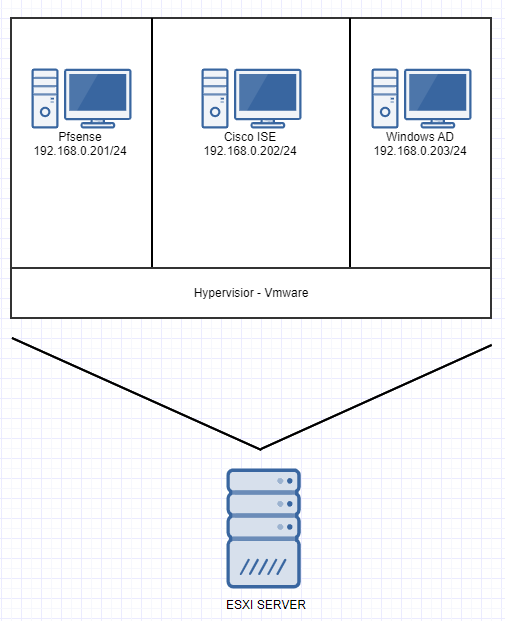
\includegraphics[height=0.3\textheight]{servervm.png}
	\caption{Deze afbeelding geeft een visueel beeld weer van de bestaande virtuele machines in de ESXi server.}
\end{figure}

\newpage
Door configuratie van deze IP instellingen, is de VMware ESXi toeganglijk via de webbrowser. Bovendien is de hard disk drive ingesteld als raid 10. Raid 10 is een hybride combinatie tussen raid 1 en raid 0. Waarbij men de snelheid van striping met de veiligheid van mirroring combineert. 
\newline
\newline
Dit is de veiligste en snelste methode maar ook de duurste. Het is een dure methode omdat er gebruik wordt gemaakt van raid 1, dus voor iedere 1TB aan opslagruimte is er ook 1TB aan mirror ruimte nodig, in combinatie met raid 0 waardoor er veel schijven nodig zijn. 

\begin{figure}[H]
	\centering
	\includegraphics[height=0.25\textheight]{Raid10.png}
	\caption{Deze afbeelding geeft een visueel beeld weer van een RAID 10 configuratie.}
\end{figure}

In deze server opstelling zijn drie van de vier fysieke ethernet adapters gebruikt. Deze adapters zijn op hun beurt verbonden met een virtuele switch. Elk van deze fysieke adapter heeft een andere functie. Deze functies zijn terug te vinden in onderstaande lijst. 

\begin{itemize}
	\item vmnic0,is de fysieke adapter die verbonden is met de virtuele switch, genaamd 'VSwitch0'.
	\item vmnic2,is de fysieke adapter die verbonden is met de virtuele switch, genaamd 'Sub\textunderscore switch'.
	\item vmnic3,is de fysieke adapter die verbonden is met de virtuele switch, genaamd 'Cisco \textunderscore switch'.
\end{itemize}

\newpage
\subsubsection{Virtuele switches}
\subsubitem{\bf VSwitch0}
\newline
De 'VSwitch0' is een virtuele switch die voorzien is om de VMware ESXi te contacteren via de webbrower. Deze switch is ingesteld met vlan id 0. Dit betekent m.a.w. dat hiervoor geen vlan identificatie is voorzien. 
\newline
\newline
Wanneer gebruikers surfen naar "https://192.168.0.183/", dan passeert deze data langs de fysieke poort vmnic0. Vervolgens stuurt de fysieke poort de data door naar de VSwitch0. Wanneer de data op de VSwitch0 terecht komt, stuurt hij op zijn beurt de data door naar de VMKernel poort.

\begin{figure}[H]
	\centering
	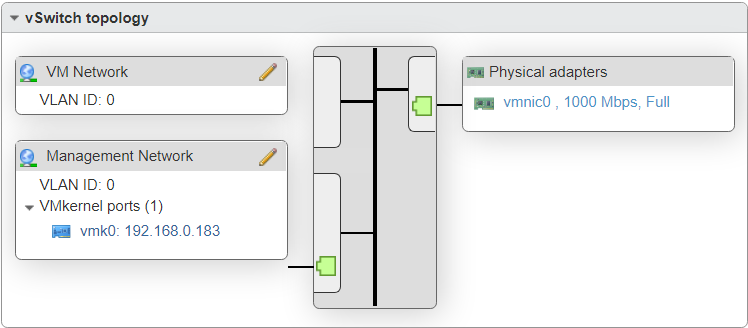
\includegraphics[width=0.7\textwidth]{VSwitch0.png}
	\caption{Deze afbeelding geeft een visueel beeld weer van de 'VSwitch0' topologie.}
\end{figure}

\subsubitem{\bf Sub\textunderscore switch}
\newline
De 'Sub\textunderscore switch' is een virtuele switch die gebruikt wordt als WAN interface voor de Pfsense. De WAN interface voorziet data overdracht van de thuis LAN netwerk naar het afgezonderd LAN netwerk. M.a.w. is connectie met het afgezonderd netwerkje mogelijk via deze interface. Bovendien is deze virtuele switch ook gebruikt voor de jumphost. Deze jumphost maakt het mogelijk om remote desktop protocol connecties te maken met de virtuele machines binnen het afgezonderd netwerkje. 
\newline
\newline
Vervolgens is deze virtuele switch ook ingesteld met vlan id 0. Dit betekend m.a.w. dat hiervoor geen vlan identificatie is voorzien. 

\begin{figure}[H]
	\centering
	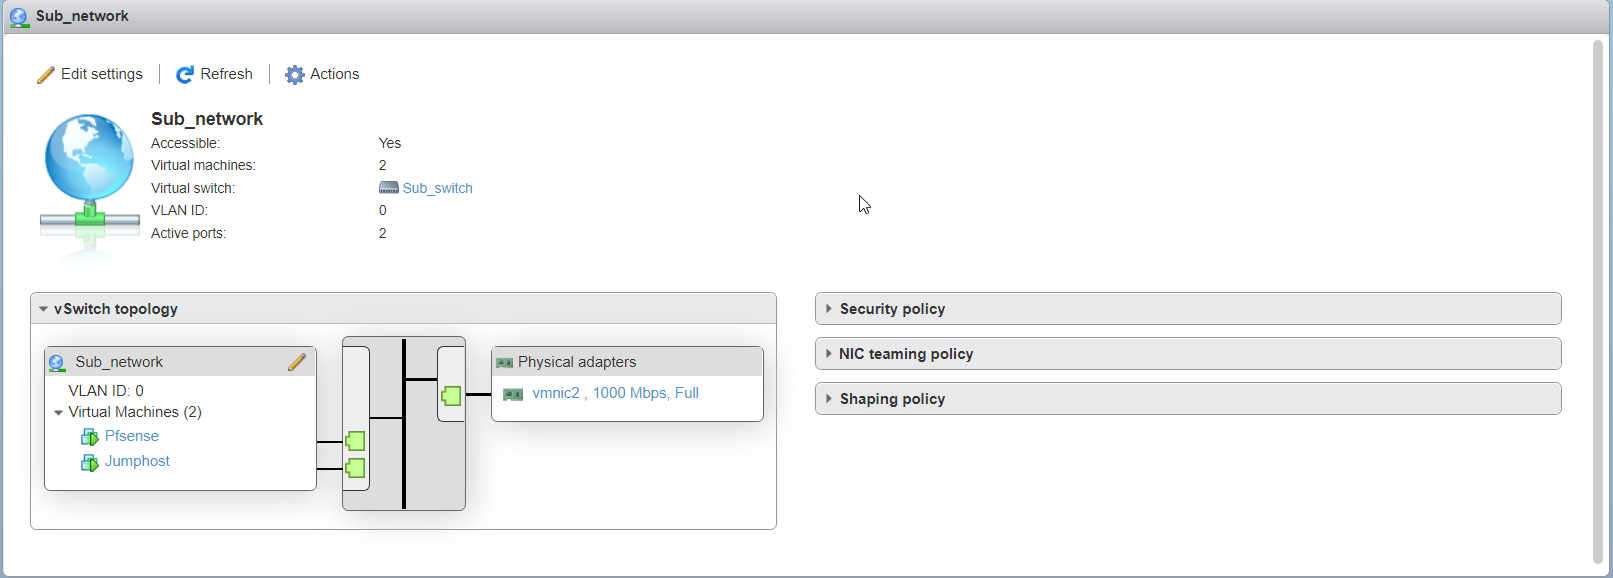
\includegraphics[width=0.7\textwidth]{Subswitch.png}
	\caption{Deze afbeelding geeft een visueel beeld weer van de 'Sub\textunderscore switch' topologie.}
\end{figure}

\subsubitem{\bf Cisco\textunderscore switch}
\newline
De 'Cisco\textunderscore switch'  is terug een virtuele switch. Deze switch wordt gebruikt om connectie te maken met alle apparaten achterliggend de fysieke Cisco switch. Dit betekent wanneer eind apparaten met de Cisco switch verbinden, dan zal de data passeren via deze virtuele switch. Bovendien bevinden alle andere virtuele machine zich in deze omgeving. Met als gevolgd is deze virtuele switch  ingesteld met vlan id 10. Dit betekent dat enkel data vanuit vlan 10 wordt doorgestuurd naar de voorziene machines.

\begin{figure}[H]
	\centering
	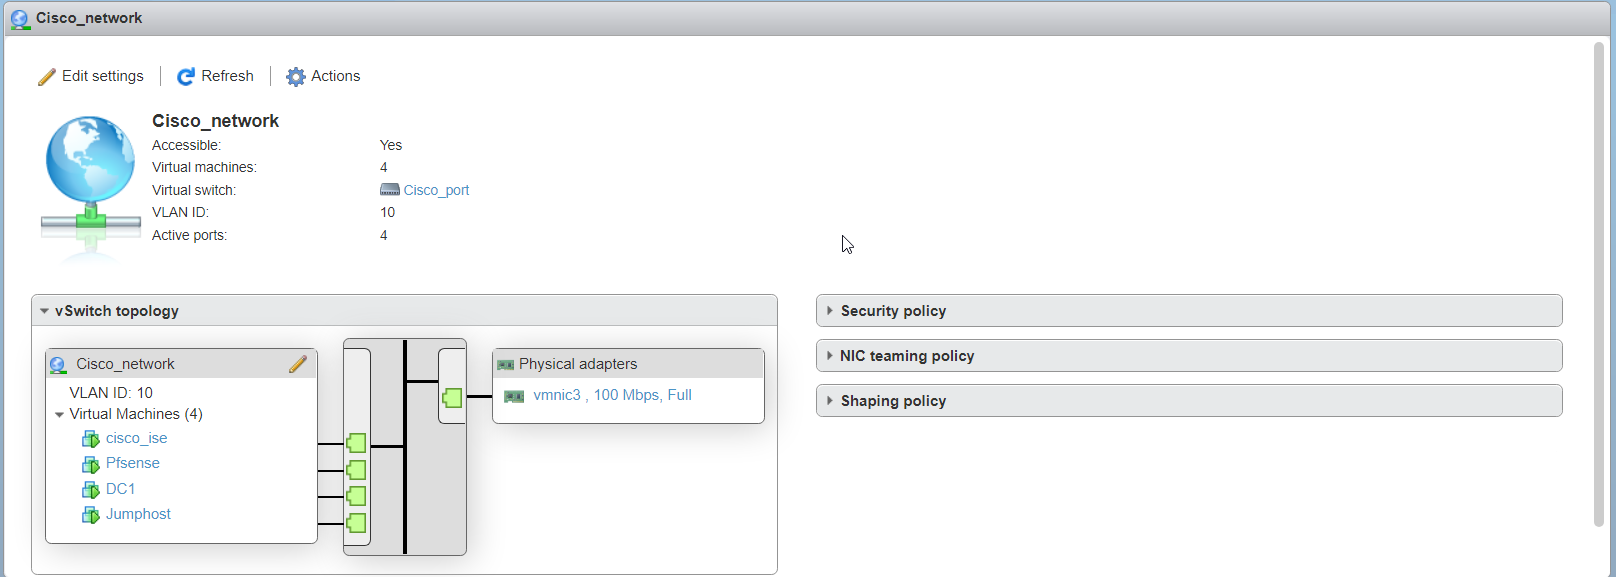
\includegraphics[width=0.7\textwidth]{CiscoSwitch_vmware.png}
	\caption{Deze afbeelding geeft een visueel beeld weer van de 'Cisco\textunderscore switch' topologie.}
\end{figure}

\subsubsection{Server ESXi specificaties}
De voorziene ESXi server is van het merk International Business Machines Corporation, gekend als IBM. Deze server werd oorsprongelijk gebruikt in de productie omgeving van Axians, maar is sinds kort een test server. 
\newline
\newline
Hierbij heeft ‘System x3350 M3’, gekend binnen Axians als ‘de oude shr-esx-04 server’, de volgende specificaties:

\begin{itemize}
	\item Vormfactor: 1U Rack
	\item Processor:
	\begin{itemize}
		\item Proccessorsnelheid: 2.53GHz
		\item Processor: 6-core processor
	\end{itemize}
	\item Geheugen:
	\begin{itemize}
		\item Intern geheugen: 240 GB Random Access Memory
		\item Intern geheugentype: Double Data Rate 3 Synchronous Dynamic Random-Access Memory, gekend als DDR3 SDRAM
	\end{itemize}
	\item Opslag:
	\begin{itemize}
		\item Maximum aantal schrijven: 8 Slots
		\item Opslag: 4 Terabyte HHD 7500 RPM
	\end{itemize}
	\item Netwerk
	\begin{itemize}
		\item Ethernet interface type: Gigabit Ethernet
		\item Aantal ethernet poorten: 4 
	\end{itemize}
\end{itemize}

\begin{figure}[H]
	\centering
	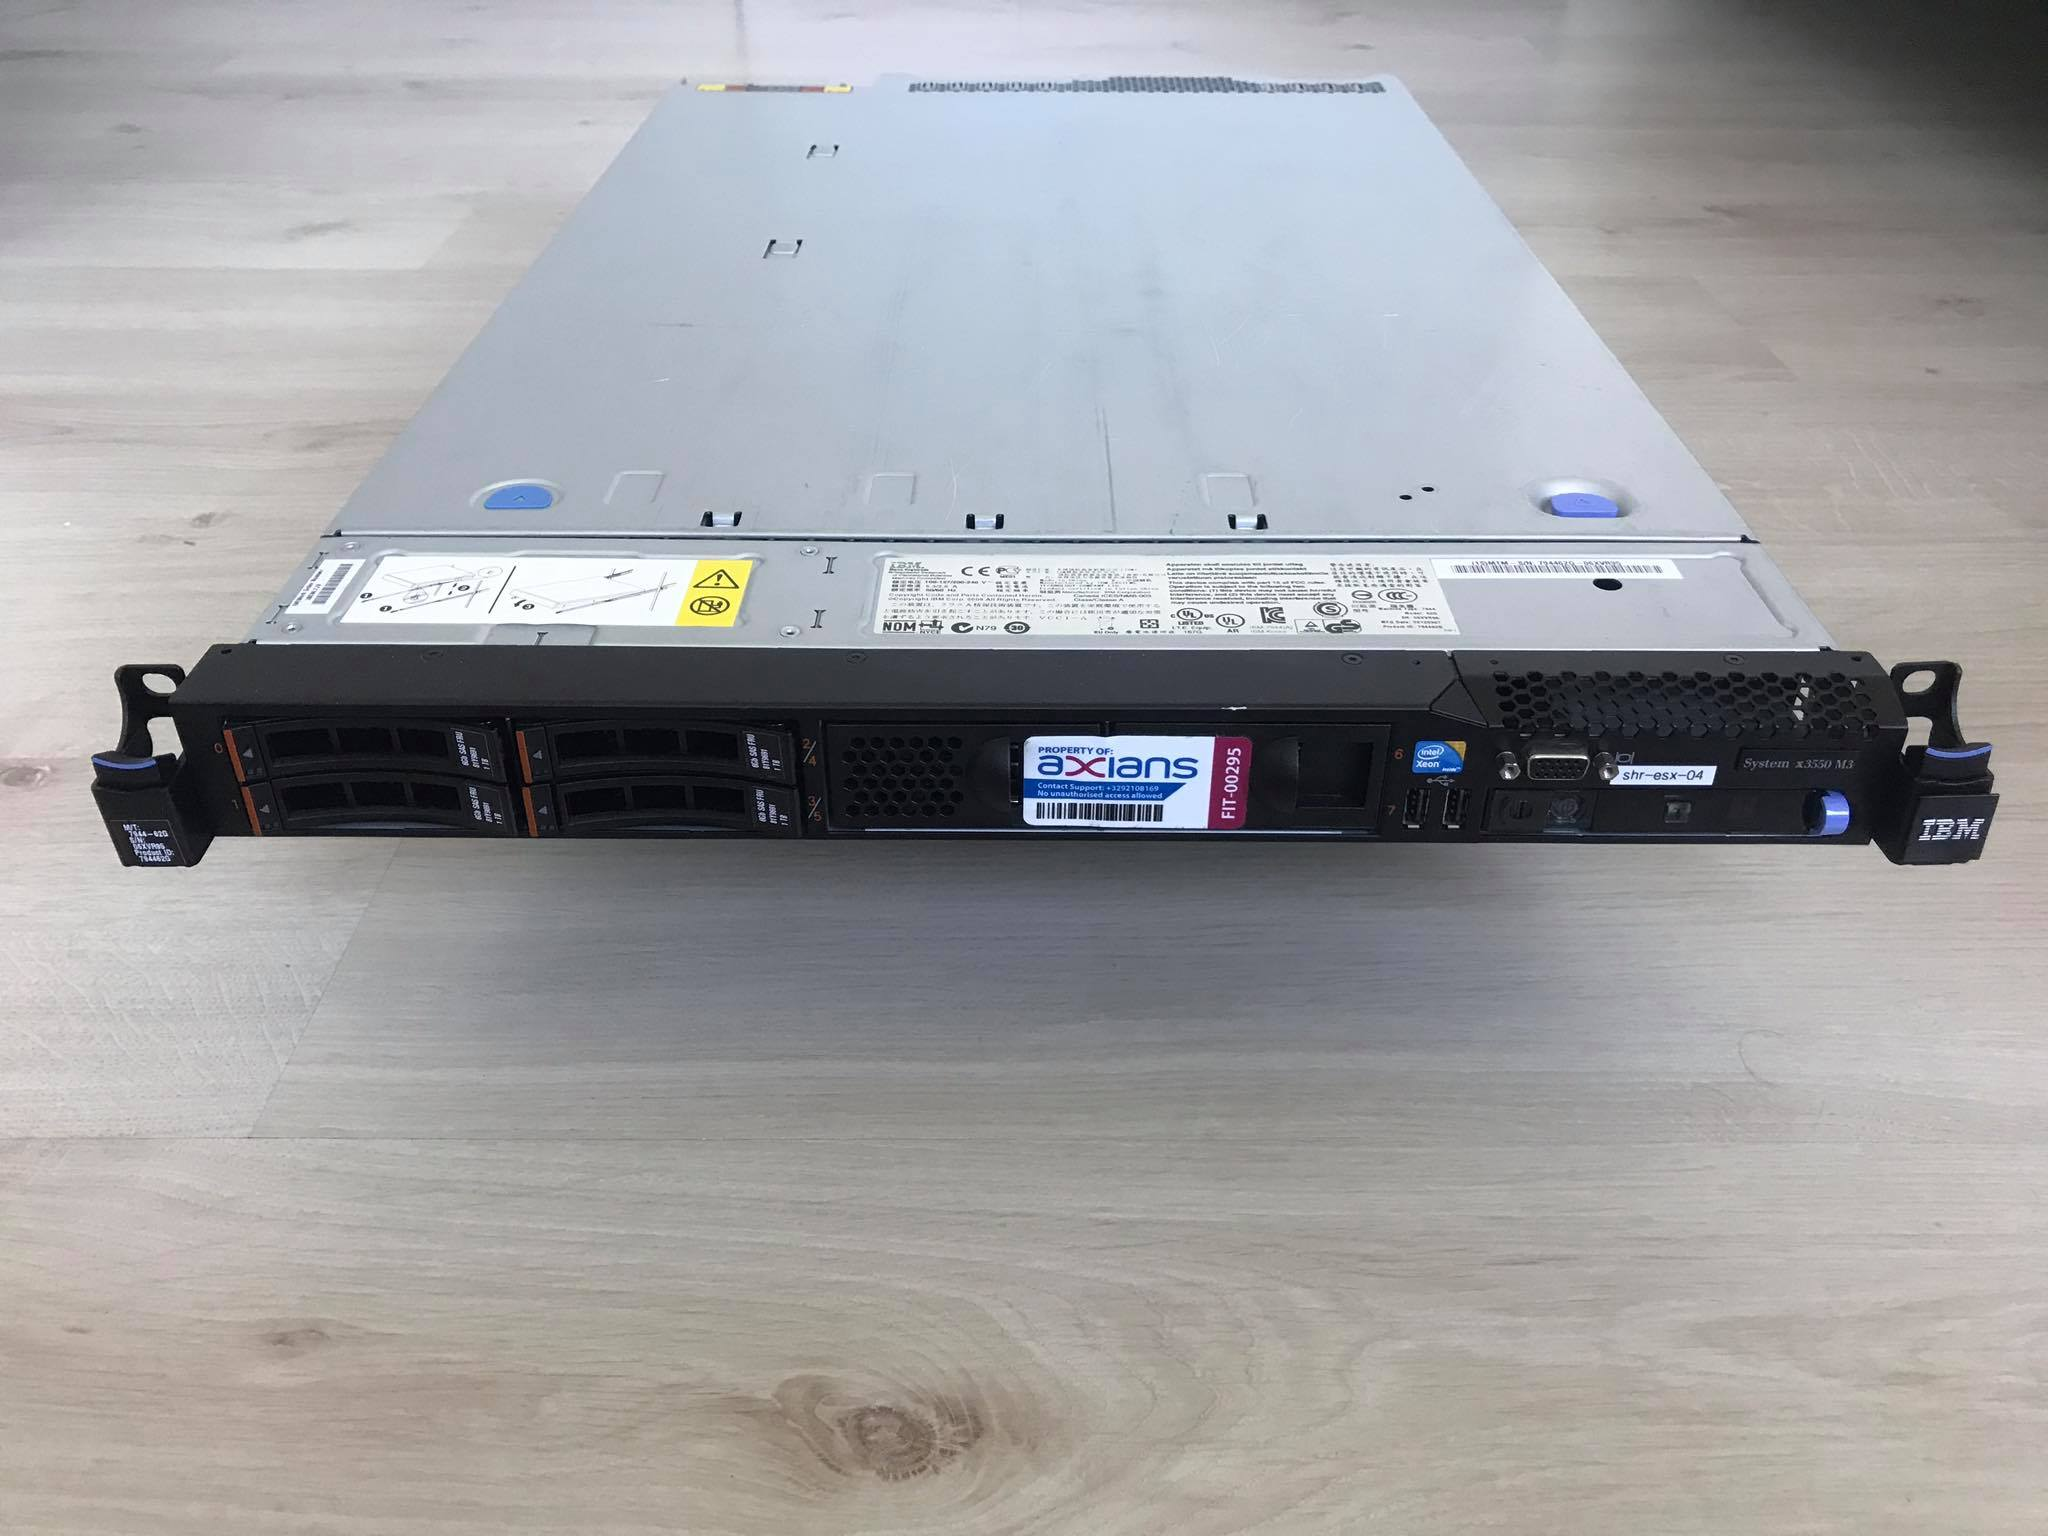
\includegraphics[width=0.5\textwidth]{serveresxi.png}
	\caption{Deze afbeelding heeft de ESXI server weer. }
\end{figure}

\subsection{Cisco switch}
Naast de ESXi server, bestaat de Cisco Identity Services Engine omgeving ook uit een Cisco switch. Deze fysieke switch werd geconfigureerd, zodanig dat de Cisco Identity Services Engine virtuele machine kan communiceren met deze switch. Om deze communicatie mogelijk te maken, zijn er bepaalde configuraties uitgevoerd op deze fysieke switch. Deze noodzakelijke configuraties speelden een belangrijke rol in de configuratie van de 'Port-based network access control' use case. 
\newline
\newline
Daarnaast zijn er ook een aantal basis configuraties uitgevoerd op deze switch. Hierdoor wordt communicatie tussen het afgezonderd netwerk en de eind apparaten achterliggend de switch ook mogelijk. Deze informatie is terug te vinden in de volgende subsectie.  

\subsubsection{Configuratie}
Om te beginnen werd de Cisco switch met een aantal commando's geconfigureerd. Deze configuraties beveiligen het network apparaat. M.a.w. zijn secrets, line password en passwords enqryption commando's uitvoert om inbreuk tegen te gaan. 
\newline
\newline
Om te communiceren met het afgezonderd netwerk, werd Gigabit Ethernet 0/1 geconfigureerd met volgende settings: 

\begin{itemize}
	\item switchport mode trunk
	\item switchport trunk allow vlan 10 
\end{itemize}

Deze configuratie maakt data overdracht van de verschillende vlan's mogelijk. Deze poort werd rechtsverbonden met één van de interfaces op de ESXi server. Vervolgens werd een vlan gecreeërt en kreeg het ip adres '192.168.17.5' met subnet mask '255.255.255.0' toegewezen. Deze instellingen behoorde tot de basis configuratie van de Cisco switch.

\begin{figure}[H]
	\centering
	\subfloat{{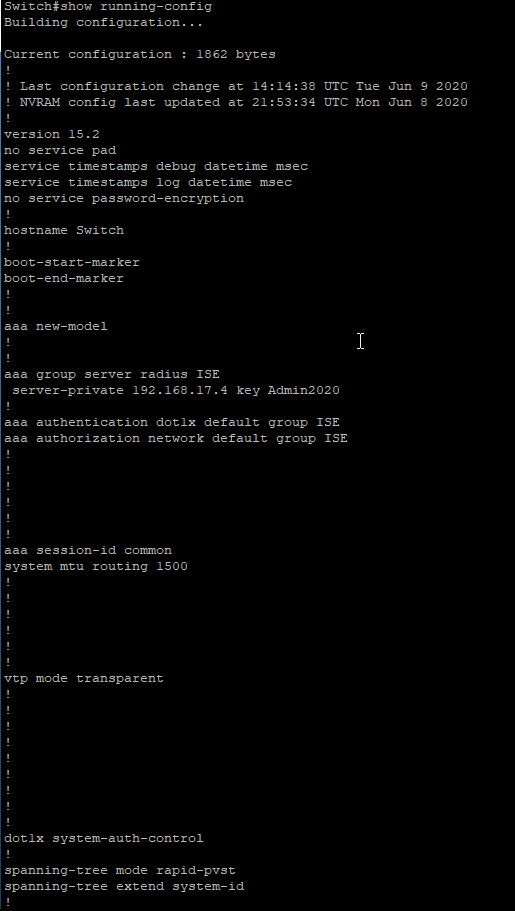
\includegraphics[width=3cm]{Switch_config1.png} }}%
	\qquad
	\subfloat{{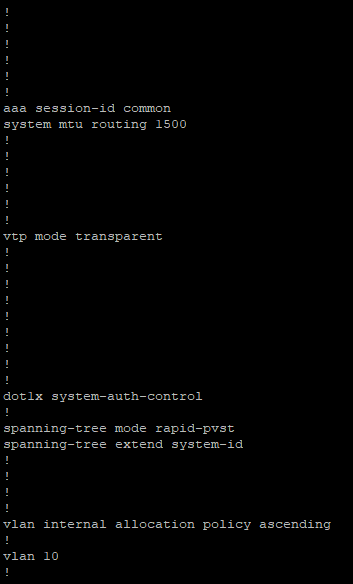
\includegraphics[width=3cm]{Switch_config2.png} }}%
	\qquad
	\subfloat{{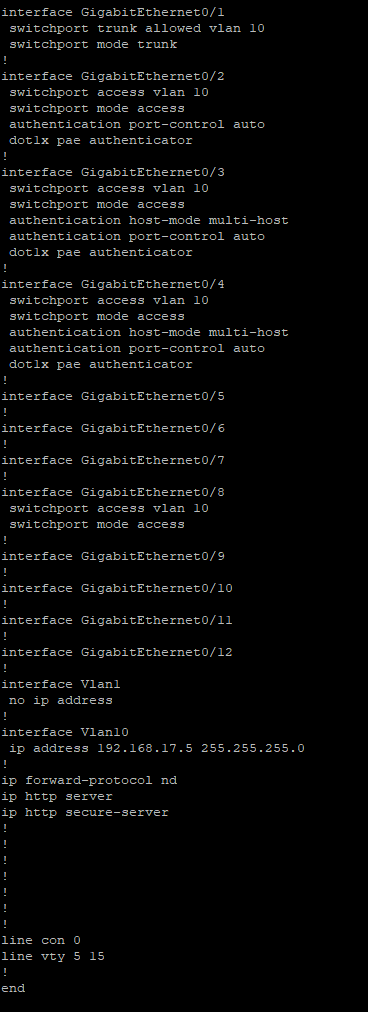
\includegraphics[width=3cm]{Switch_config3.png} }}%
	\caption{Bovenstaande foto's geven de running-config van de Cisco switch weer. Waarbij een aantal interfaces geconfigureerd zijn met het 'Policy-based network access control' use case.}%
	\label{fig:RunningConfig}%
\end{figure}

Vermits poort Gigabit Ethernet 0/1 geconfigureerd is om verbinding te maken met de server ESXi, zijn de overige poorten bedoeld voor de communicatie met de eind apparaten. Met als gevolg dat alle overige poorten ingesteld zijn met het 'Port-based network access control' use case.
\newline
\newline
Om de 'Port-based network access control' use case mogelijk te maken, werd een nieuw AAA model ingesteld. Vervolgens werd dit AAA model met een radius server geïnitialiseerd. De dot1x aaa authentication methode werd met zijn standaard netwerk group mee configureerd. 
\newline
\newline
Dot1x system-auth-control werd hierbij mee vastgelegd. Om de configuratie te beëindeigen, werden alle poorten voorzien van de nodige 'Port-based NAC' configuraties. Deze configuraties zijn in de volgende lijst weergegeven.

\begin{itemize}
	\item \#enable
	\item \#config t
	\item (config)\#aaa new-model
	\item (config)\#aaa group server radius ISE
	\item (config-sg-radius)\#server-private 192.168.17.4 key Admin2020
	\item (config-sg-radius)\#exit
	\item (config)\#aaa authentication dot1x
	\item (config)\#aaa authorization network default group ISE
	\item (config)\#dot1x system-auth-control
	\item (config)\#interface range gig0/2-12
	\item (config-if-range)\#switchport mode access
	\item (config-if-range)\#switchmode access vlan 10
	\item (config-if-range)\#authentication host-mode multi-host
	\item (config-if-range)\#authentication port-control auto
	\item (config-if-range)\#dot1x pae auth
	\item (config-if-range)\#end
\end{itemize}

\subsubsection{Communicatie}
Om deze systemen met elkaar te laten communiceren, werden 1G cat5e ethernet kabels gebruikt. Deze Unshielded Twisted Pair Ethernet kabels halen snelheden tot 1000 Mbit/s met een doorvoersnelheid van 100mhz. Wat geschikt is voor dit afgezonderd netwerk.

\subsubsection{Cisco switch specificaties}
Deze switch is van het merk Cisco Systems, en behoord tot de ‘Catalyst 2960-CX’ series. Deze Cisco switch staat nu gekend binnen Axians als de ‘Demo switch’. 
In onderstaande lijst vindt u de specificaties van de Cisco Catalyst 2960-CX serie switch:

\begin{itemize}
	\item Power over Ethernet:
	\begin{itemize}
		\item Ondersteunend: Ja
		\item Standaard: 802.3at (PoE+)
	\end{itemize}
	\item Netwerk:
	\begin{itemize}
		\item 8 Gigabit Ethernet aansluitingen
		\item 2 Gigabit Ethernet Copper uplinks
		\item 2 Gigabit Ethernet Small form-factor pluggable uplinks, gekend als SFP
	\end{itemize}
	\item Besturingsysteem/software:
	\begin{itemize}
		\item OS: Cisco IOS
\end{itemize}

\begin{figure}[H]
	\centering
	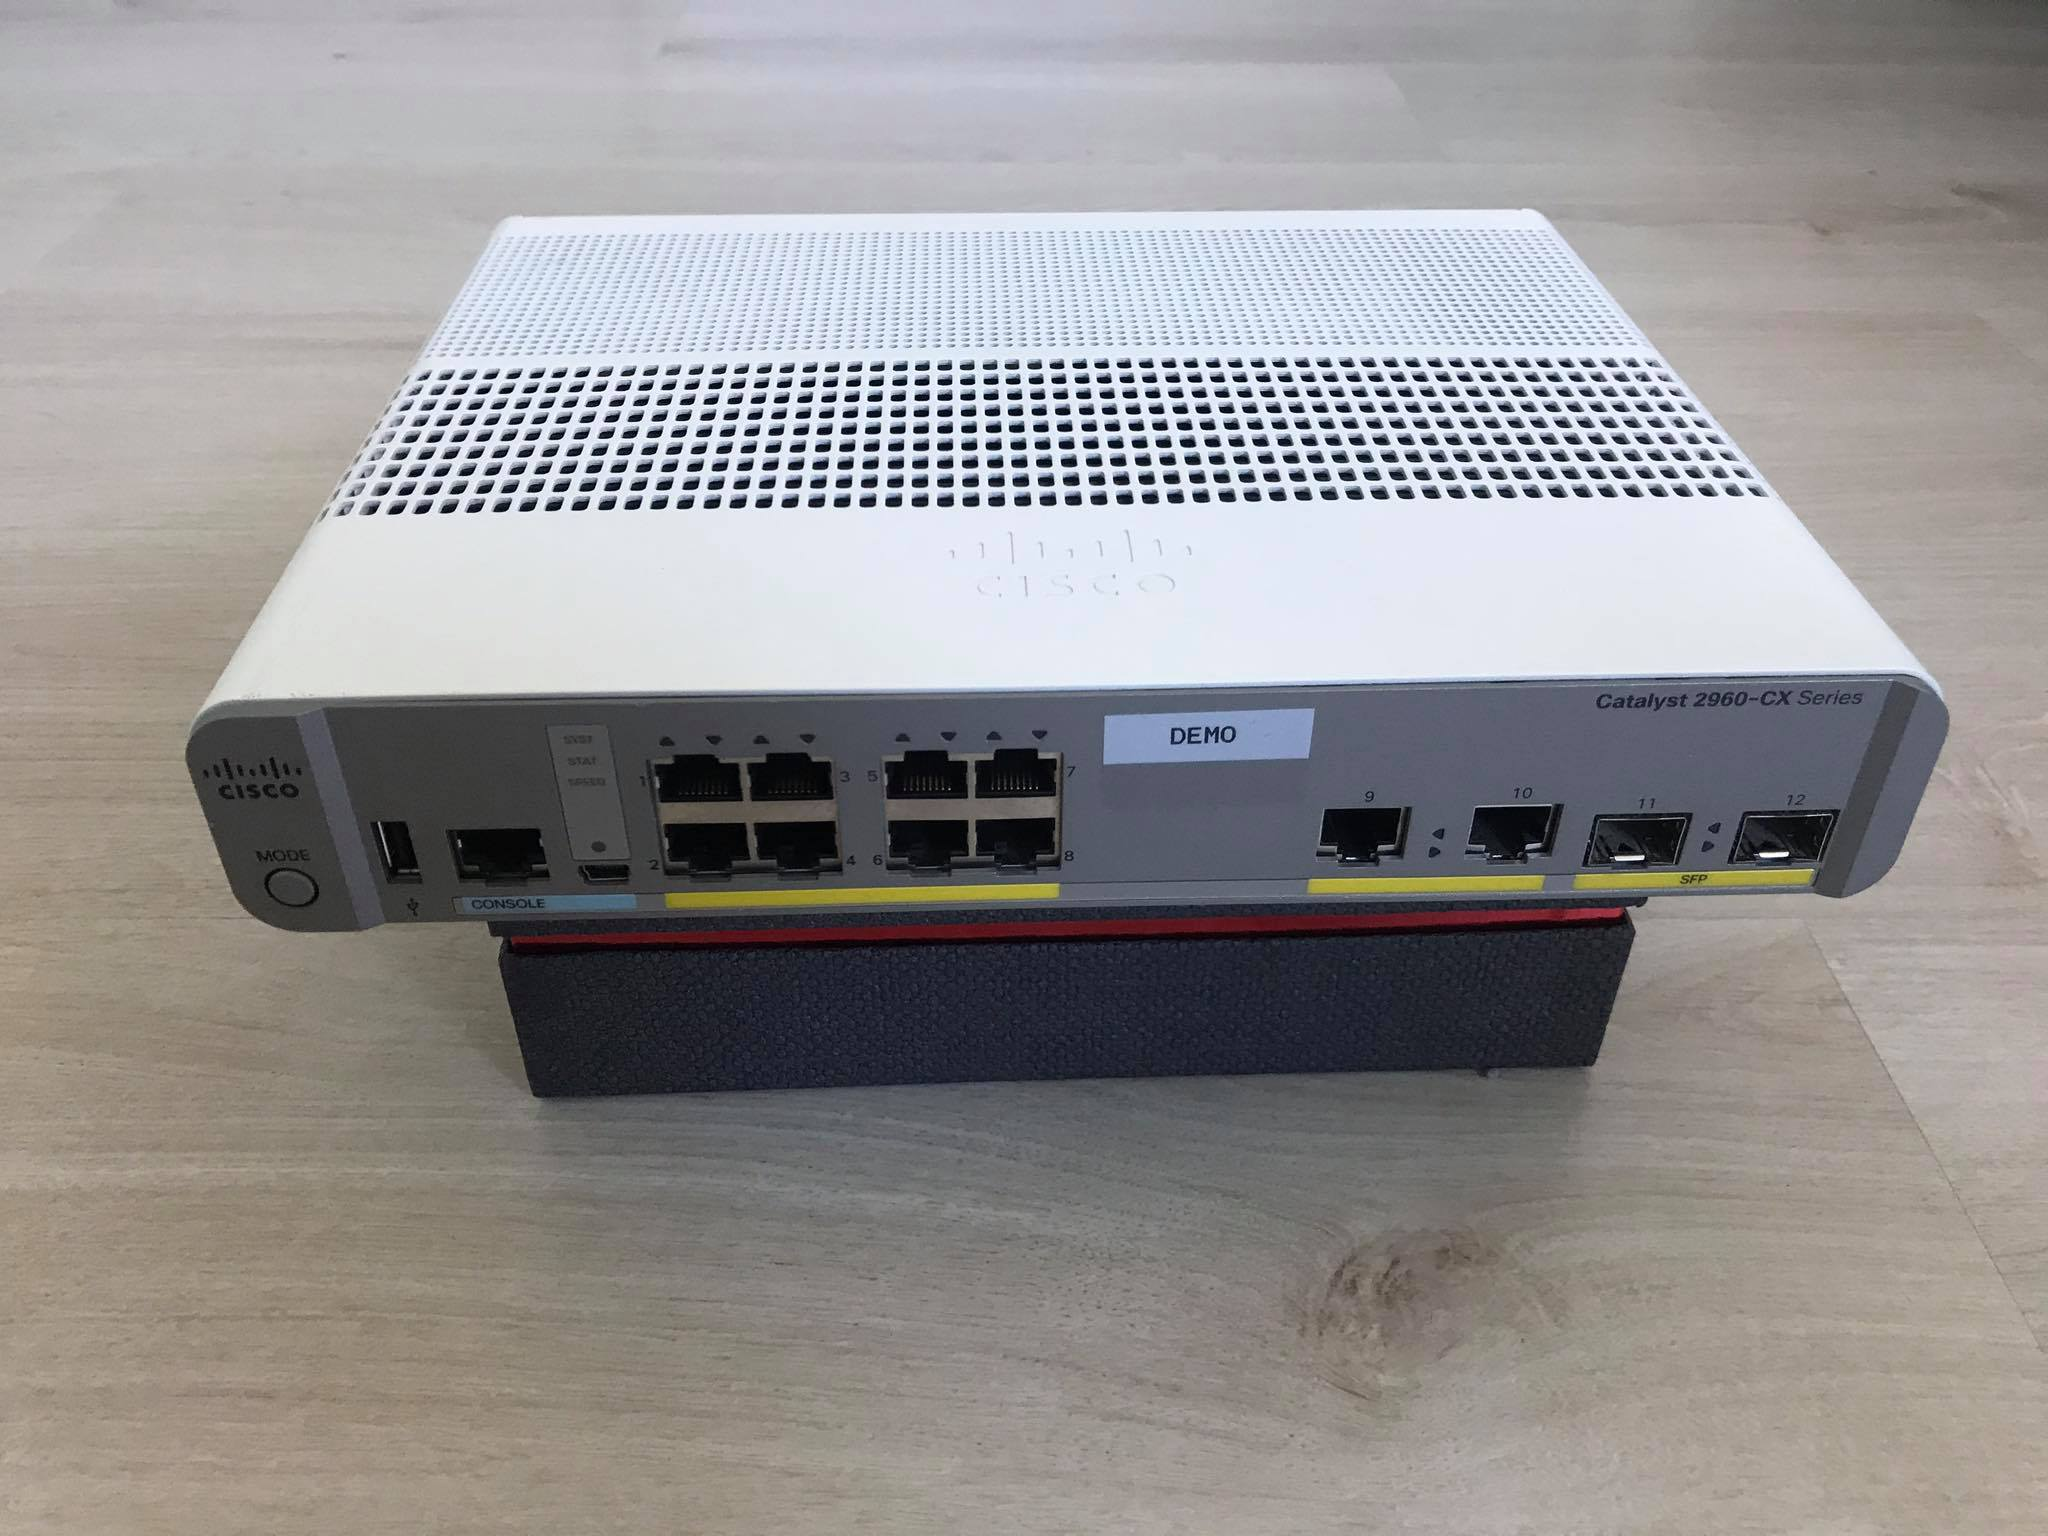
\includegraphics[width=0.5\textwidth]{ciscoswitch.png}
	\caption{Deze afbeelding heeft de Cisco switch weer. }
\end{figure}

\subsection{Virtuele machines}
\subsubsection{Cisco Identity Services Engine}
 TO DO! Praten over de omgeving en use case omgeving 
 \subsubitem{Port-based network access control}
 \subsubitem{Policy-based network access control}
 \subsubitem{Thread-centric network access control}
\newline
\newline

Dit systeem werd geïnstalleerd op een Red Hat Enterprise 7 distributie, waar vogende specificaties voor werd vrijgemaakt: 

\begin{itemize}
	\item Geheugen: 128 GB Random Access Memory
	\item Opslag: 512 GB
	\item CPU: 24 cores
	\item Netwerk adapter: Cisco\textunderscore netwerk
\end{itemize}

De installatie van Cisco Identity Services Engine werd mogelijk gemaakt door \cite{CiscoISE_InstallationGuide}.

\begin{figure}[H]
	\centering
	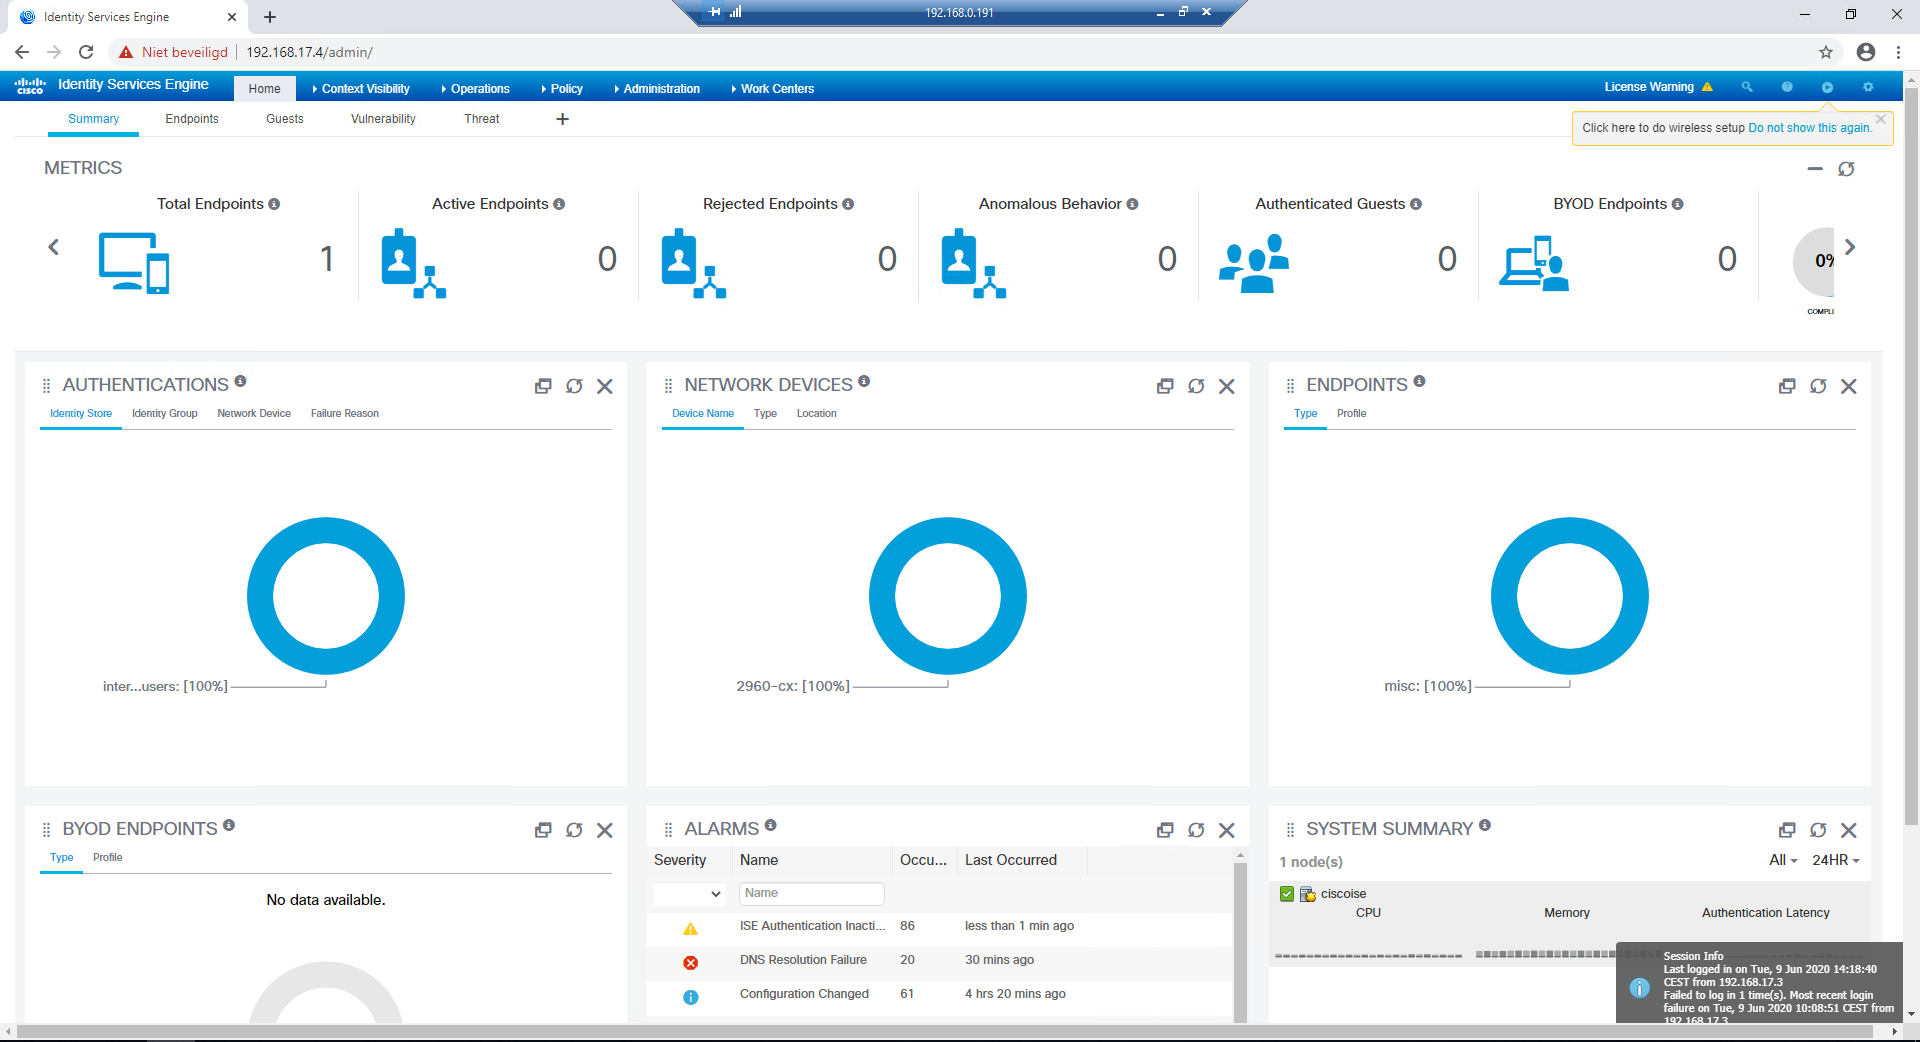
\includegraphics[width=0.5\textwidth]{homepage_ise.png}
	\caption{Deze afbeelding heeft de home page van Cisco Identity Services Engine weer.}
\end{figure}

\subsubsection{Windows server 2019 datacenter}
Op de windows server 2019 werd een Active Directory domain aangemaakt. Hiervoor werd een nieuwe forrest aangemaakt, genaamd ‘Bachelorproef.com’. Vervolgens werd deze server ook gepromoveerd naar de domaincontroller binnen het netwerk.
\newline
\newline
Via Cisco Identity Service Engine kan men subset van domeinen selecteren vanuit de vertrouwde domeinen voor authenticatie en autorisatie. Deze subset van domeinen worden authenticatiedomeinen genoemd. Het definiëren van deze authenticatiedomeinen verbetert de beveiliging door bepaalde domeinen te blokkeren, waardoor de authenticatie van de gebruikers op deze domeinen wordt beperkt.
\newline
\newline
Om dit systeem te contacteren, werd het ‘Remote Desktop Protocol (RDP)’ gebruikt met het Internet Protocol (IP) adres van dit systeem.
\newline
\newline
Dit systeem werd geïnstalleerd op een Microsoft omgeving, waar volgende specificaties voor werden vrijgemaakt:

\begin{itemize}
	\item Geheugen: 16 GB Random Access Memory
	\item Opslag: 126 GB
	\item CPU: 20 cores
	\item Netwerk adapter: Cisco\textunderscore netwerk
\end{itemize}
De installatie van Windows Server 2019 datacenter werd mogelijk gemaakt door \cite{Win19_InstallationGuide}. 

\begin{figure}[H]
	\centering
	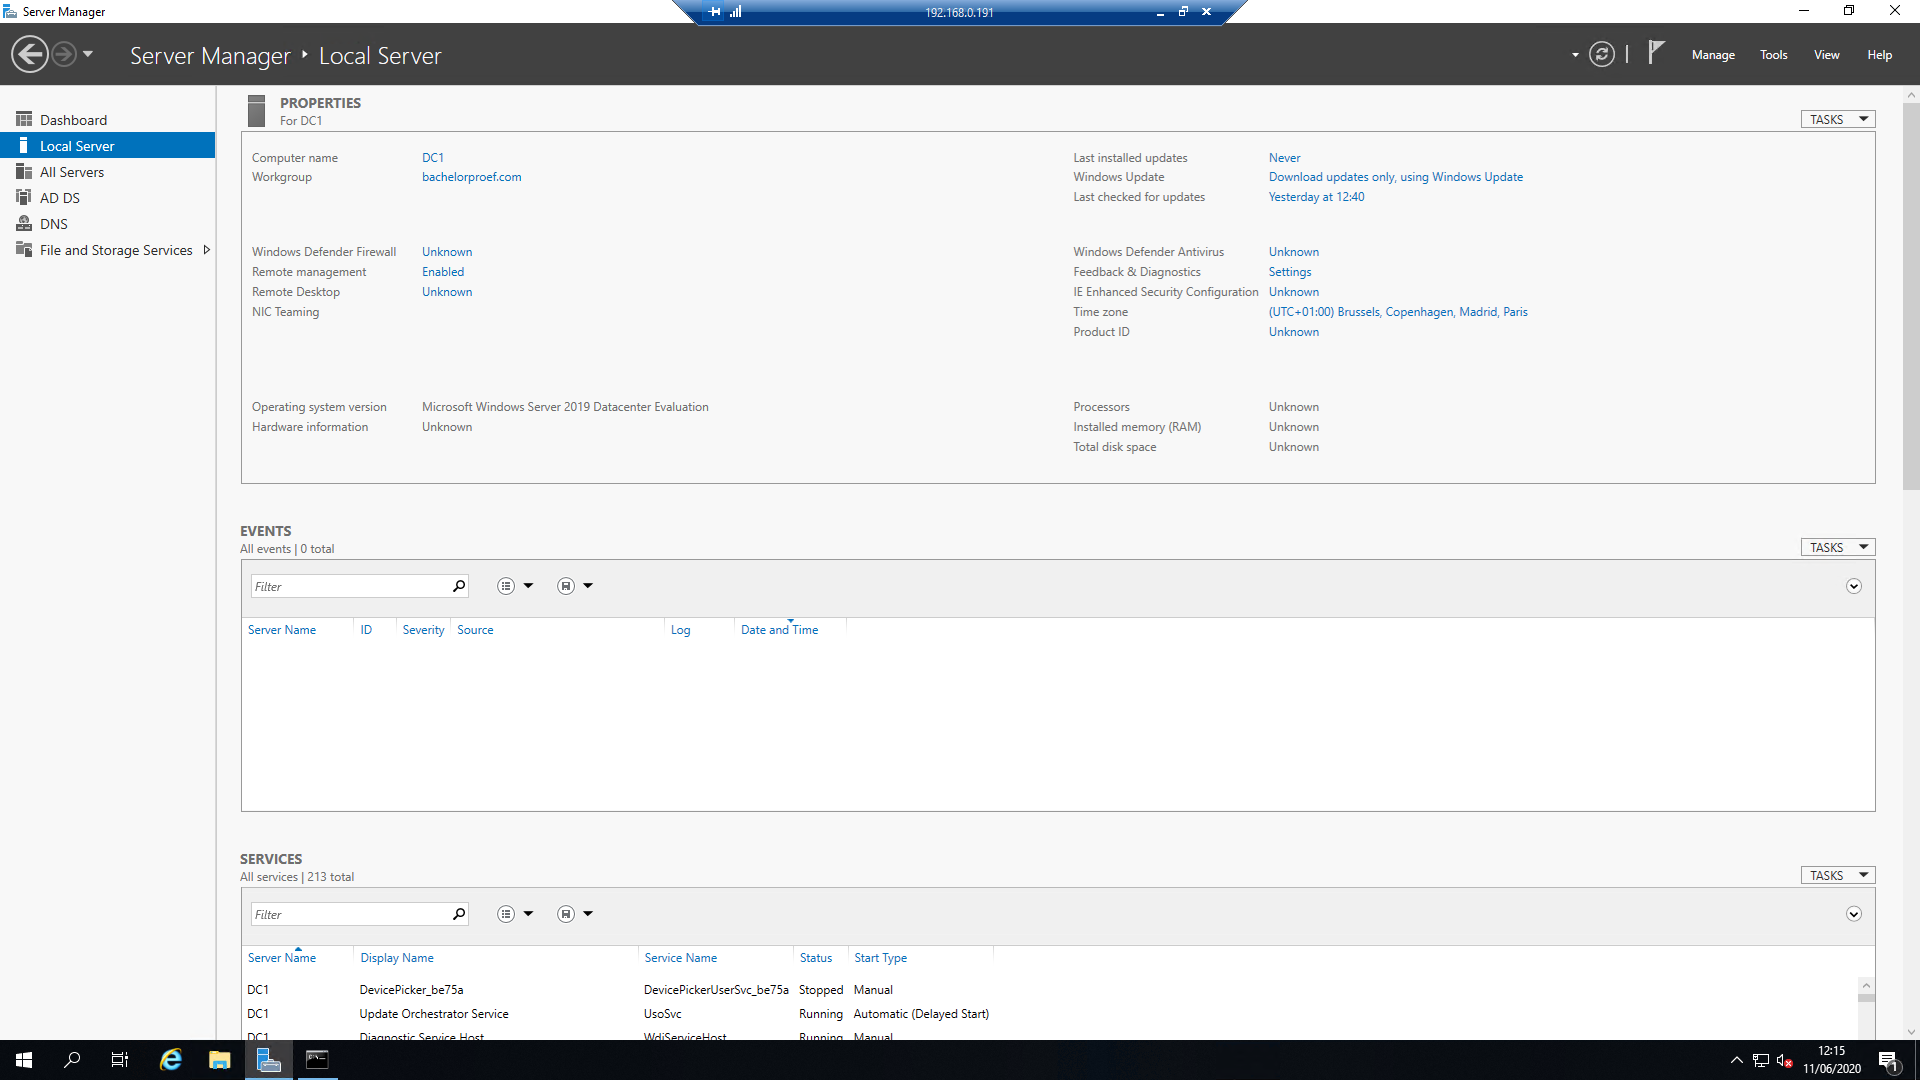
\includegraphics[width=0.6\textwidth]{WindowsHome.png}
	\caption{Deze afbeelding heeft de GUI van Windows server 2019 datacenter weer. }
\end{figure}

\subsubsection{Pfsense}
De Pfsense virtuele machine verwijst naar de virtuele router of firewall. Deze virtuele router maakt communicatie met het afgezonderd netwerk mogelijk. Zoals eerder vermeld werd deze pfsense machine gebruikt  als gateway voor alle vlan’s en alle componenten achterliggend de Cisco switch.
\newline
\newline
Om dit systeem te contacteren, werd het ‘Hypertext Transfer Protocol (HTTP)’ gebruikt met het Internet Protocol (IP) adres van dit systeem. M.a.w. werd er gesurfd naar het 'http://192.168.17.1/'.
\newline
\newline
Dit systeem werd geïnstalleerd op een FreeBSD distributie of Free Berkeley Software Distribution, waar volgende specificaties voor werd vrijgemaakt: 

\begin{itemize}
	\item Geheugen: 4 GB Random Access Memory
	\item Opslag: 25 GB
	\item CPU: 4 cores
	\item Netwerk adapter: Cisco\textunderscore netwerk
\end{itemize}
De installatie van Pfsense werd mogelijk gemaakt door \cite{Pfsense_InstallationGuide}.

\begin{figure}[H]
	\centering
	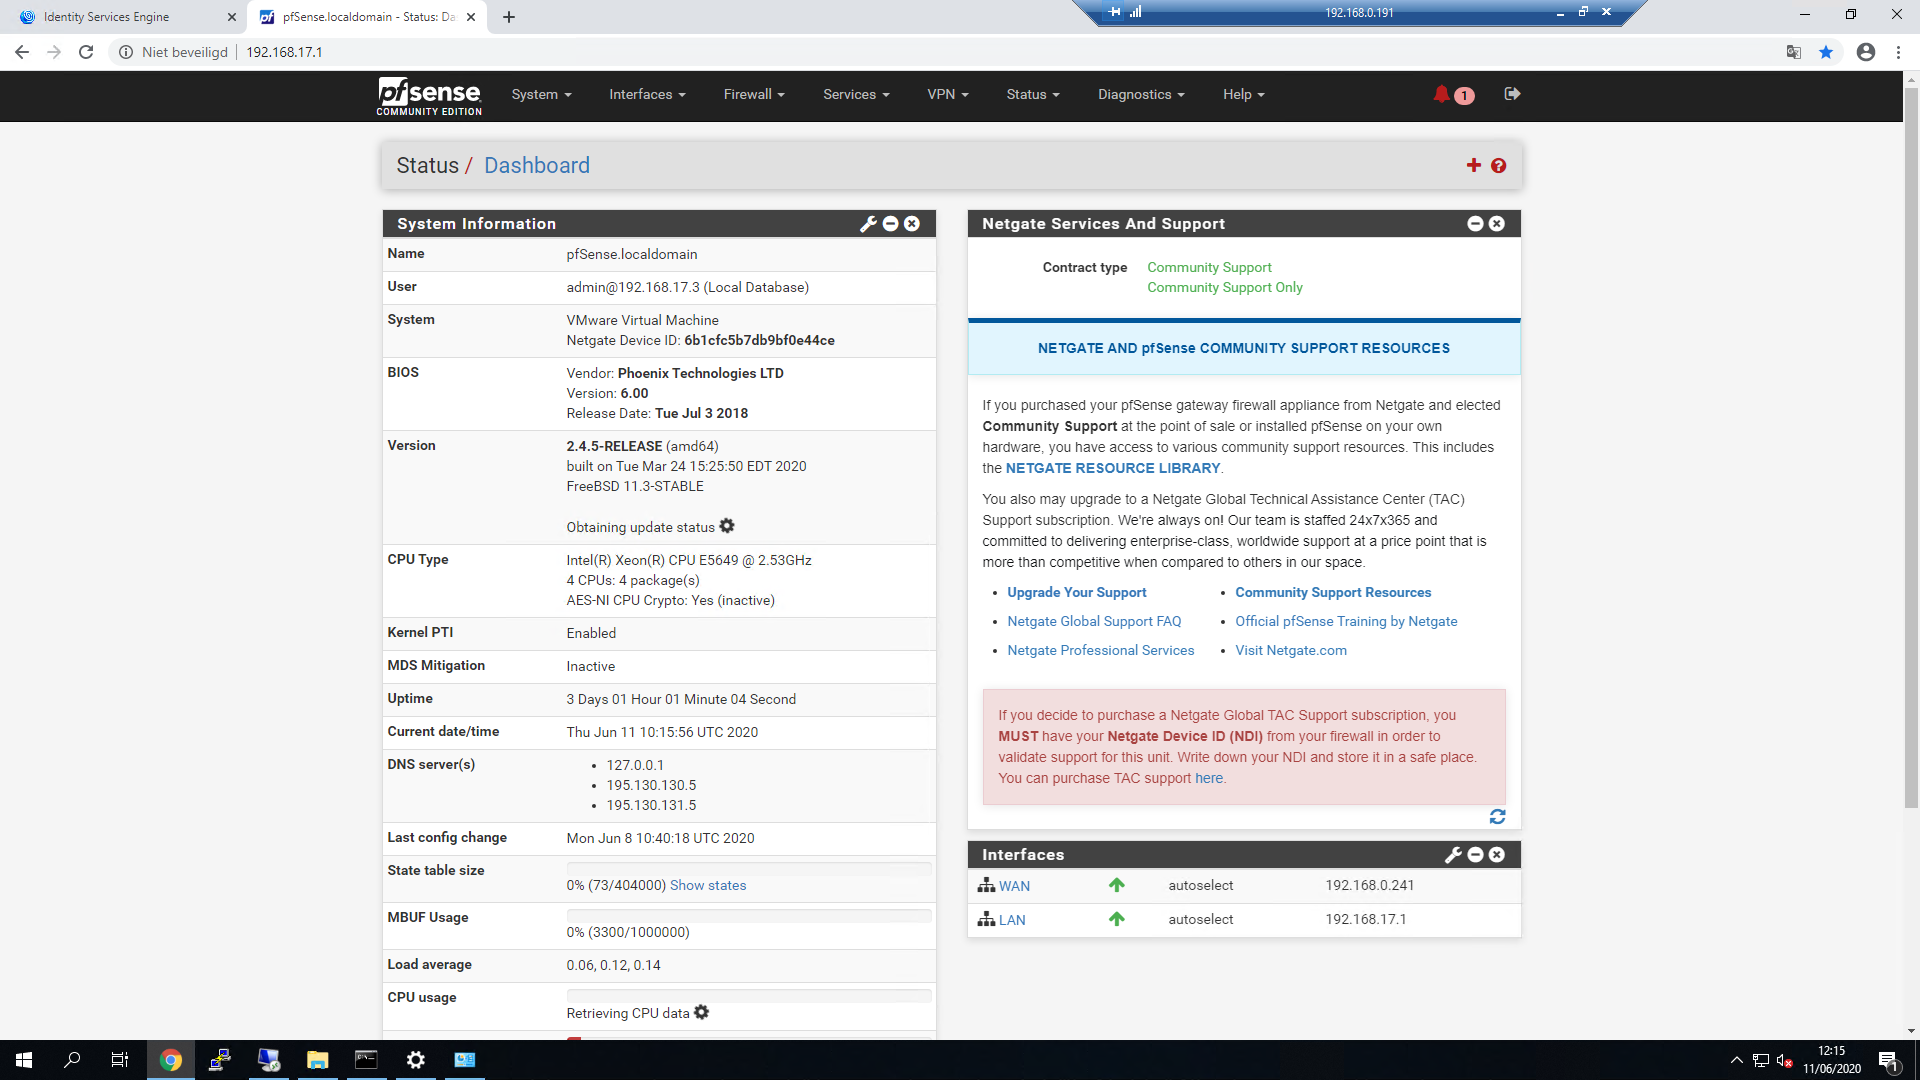
\includegraphics[width=0.6\textwidth]{PfsenseHome.png}
	\caption{Deze afbeelding heeft de GUI van Pfsense weer. }
\end{figure}

\subsubsection{Jumphost}
TO DO!

\begin{itemize}
	\item Geheugen: 16 GB Random Access Memory
	\item Opslag: 126 GB
	\item CPU: 20 cores
	\item Netwerk adapter 1: Cisco\textunderscore netwerk
	\item Netwerk adapter 2: Cisco\textunderscore netwerk
\end{itemize}

De installatie van Pfsense werd mogelijk gemaakt door \cite{Pfsense_InstallationGuide}.

\begin{figure}[H]
	\centering
	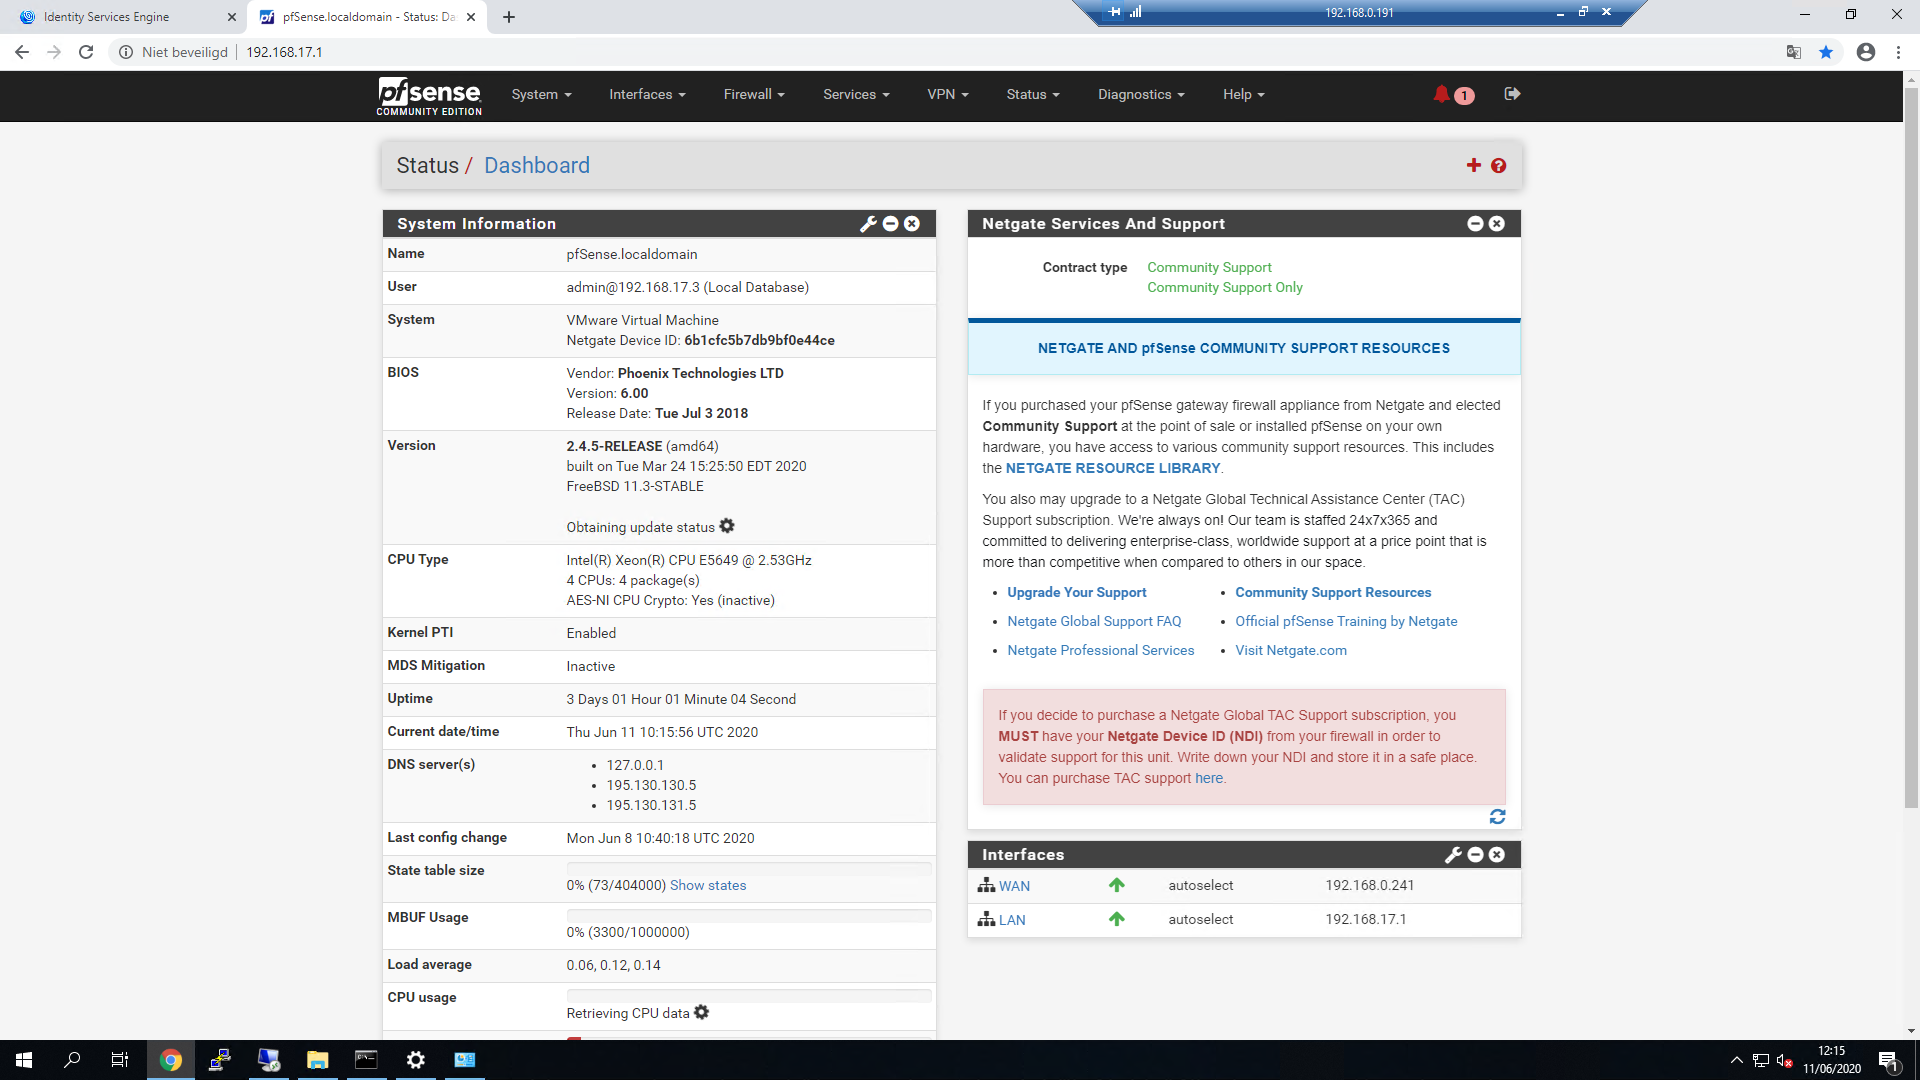
\includegraphics[width=0.7\textwidth]{PfsenseHome.png}
	\caption{Figuur 4.8 heeft de GUI van Pfsense weer. }
\end{figure}

\subsection{Begrippen}
\subsubitem{Telenet Access Point}
\newline
Een Access point is een draadloze server die gegevens verzendt via radio golven in middel van een antenne. Deze gegevens worden ontvangen via het bedrage UTP netwerk waarbij deze “server” is op aan gesloten.
\subsubitem{Telenet Modem}
\newline
Een modem is een toestel die informatie van uw internetprovider ontvangt via een telefoonlijn, glasvezelkabel of coaxkabel in de woning en converteert dit naar een digitaal signaal.
\subsubitem{Coax kabel}
\newline
Een Coax kabel een twee polige kabel die instaat voor het overdragen van beeld en geluid. Deze signalen treden gemakkelijker binnen, waarbij het signaal op korte afstanden snel zwak wordt. 
\subsubitem{Virtual local area network}
\newline
Dit is een type virtueel network dat gerealiseerd wordt op de datalinklaag. Dit bestaat uit een groep eindstations en switches die logisch gezien één enkel gemeenschappelijk local area network (LAN) vormen.

\begin{figure}[H]
	\centering
	\subfloat{{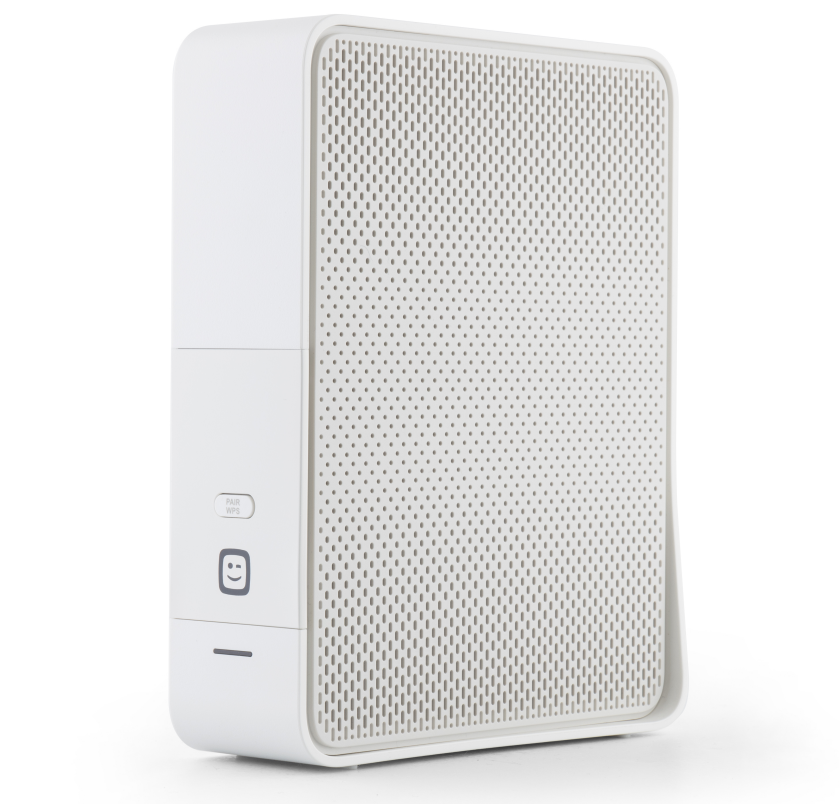
\includegraphics[width=5cm]{TelenetAP.png} }}%
	\qquad
	\subfloat{{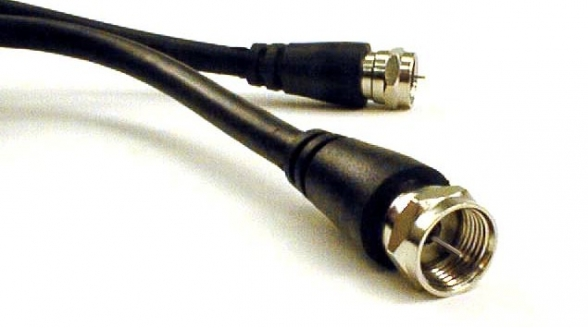
\includegraphics[width=5cm]{Coaxkabel.png} }}%
	\caption{De foto aan de linkerkant is een voorbeeld van een Telenet access point. De foto aan de rechterkant is een voorbeeld van een Coaxkabel.}%
	\label{fig:example}%
\end{figure}

\newpage
\section{Cisco Identity Services Engine enquête}
Om een link te leggen met de resultaten van de uitgevoerde testen, werd een enquête of een formulier opstelt. Deze enquête is als onderliggende basis gebruikt bij de analyse van de resultaten die verkregen werden door de fysieke testen. Zoals in vorige hoofdstukken vermeld, is deze enquête een opiniepeiling. Waarbij een aantal vragen gesteld zijn aan personen die reeds gekend zijn met Cisco Identity Services Engine. Hierdoor is de doelgroep van deze enquête beperkt tot de Cisco Identity Services Engine specialisten.
\newline
\newline
Deze enquête is publiekelijk gemaakt via LinkedIn en via E-mail. Linkedin is een online sociaal netwerk dat is opgericht voor Vakmensen, die ongeveer 610 miljoen geregistreerden telt. Omdat deze enquête publiekelijk werd gemaakt op \cite{LinkedIn}, bevat dit formulier een aantal ‘failsave’ vragen. Deze ‘failsave’ vragen zijn bedoelt wanneer niet Cisco Identity Services Engine specialisten de enquête proberen in te vullen. Met als gevolg dat de kans op onjuiste ingevuld antwoorden verkleind werd.
\newline
\newline
Dit formulier of enquête werd mogelijk gemaakt door Microsoft en Hogeschool Gent. Elke student heeft recht op een gelicentieerd Office 365 pakket gedurende zijn opleidingstraject. Het programma in kwestie noemt men \cite{MicrosoftForms} dat inbegrepen is in het Microsoft Office 365 pakket.
\newline
\newline
Hieronder vindt u een overzicht van de vragen die gesteld werden tijdens de enquête. Bij elke vraag is steeds een klein woordje uitleg gegeven. Idem zoals de mogelijke antwoorden en eventuele doorverwijzingen naar andere vragen.

\newpage
\subsection{De enquête vragen}
\textbf{Vraag 1 : Ken u Cisco Identity Services Engine?}
\newline
Antwoord 1: Ja. \newline
Antwoord 2: Neen. \newline \newline
Wanneer men bij deze vraag ‘Neen’ antwoord, dan komt men uit bij vraag 3. Het is enkel wanneer men ‘Ja’ antwoord dat er wordt overgegaan naar vraag 2.

\textbf{Vraag 2: Waar heeft u voor het eerst gehoord van Cisco Identity Services Engine?}
\newline
Antwoord 1: Tijdens een webinair. \newline
Antwoord 2: Tijdens een opleiding. \newline
Antwoord 3: In de organisatie. \newline
Antwoord 4: Op het internet. \newline
Antwoord 5: Op een reclame campagne. \newline
Antwoord 6: Op televisie. \newline
Antwoord 7: Andere \newline \newline
Na het invullen van deze vraag wordt er overgegaan naar vraag 3. Bij deze vraag is slechts één antwoord mogelijk. 

\textbf{Vraag 3: Wordt Cisco Identity Services Engine binnen uw organisatie toegepast?}
\newline
Antwoord 1: Ja.\newline
Antwoord 2: Neen.\newline \newline
Wanneer men antwoord op deze vraag met ‘Neen’. Dan wordt er overgaan naar de volgende vraag, anders springt men naar vraag 6.

\textbf{Vraag 4: Wordt er een network access control product gebruikt in uw organisatie? }
\newline
\textit{Ondertekst: Bijv: Portnox , Auba Clearpass, Cisco ISE, etc. }\newline
Antwoord 1: Ja.\newline
Antwoord 2: Neen.\newline \newline
Deze vraag is enkel bereikbaar wanneer er op vorige vraag geantwoord wordt met ‘Neen’. Deze vraag is bedoelt wanneer ‘niet Cisco Identity Services Engine specialisten’ de enquête invullen. Vervolgens is direct ook duidelijk of dat men al dan niet een network access control product toepast in hun bedrijfsomgeving. 

\textbf{Vraag 5: Welk network access control product wordt in uw organisatie gebruikt?}
\newline
Via deze vraag wordt er duidelijkheid geschept over het type network access control product wordt toegepast in de omgeving van de geënquêteerde. Hiervoor werd een open vraag gesteld. Het is enkel wanneer er op vorige vraag geantwoord wordt met ‘Ja’, dat er overgegaan wordt naar deze vraag. Indien men ‘Neen’ antwoord, dan springt de enquête naar vraag 7. 

\newpage
\textbf{Vraag 6: Met welke reden werd Cisco Identity Services gekozen als network access control in uw bedrijfsomgeving?}
\newline
Antwoord 1: Omwille van Cisco’s bedrijfsimage. \newline
Antwoord 2: Omwille van de betere beschermingen tegen interne of externe threads t.o.v. andere network access control producten. \newline
Antwoord 3: Omwille van de betere zichtbaarheid en de nauwkeurigheid voor apparaatidentificatie t.o.v. andere network access control producten. \newline
Antwoord 4: Omwille van de betere beheerbaarheid van end-point systemen t.o.v. van andere network access control producten. \newline
Antwoord 5: Andere. \newline \newline

Via deze vraag wordt de rede waarom de geënquêteerde koos voor Cisco Identity Services Engine als network access control product binnen hun opgeving. Deze vraag is enkel toeganglijk wanneer men antwoord op vraag drie met ‘Ja’.

\textbf{Vraag 7: Welke kernmerken zijn volgens u belangrijk om te kiezen voor een network access control product?}
\newline

TO DO!!

\textbf{Vraag 8: Ondervond u na de implementatie van Cisco Identity Services Engine enige veranderingen? Zoja, welke?}
\newline
\textit{Ondertekst: Bijv: Sinds de implementatie van Cisco ISE worden minder endpoint systemen besmet met malware door de overdracht van laptops. Wat voordien af en toe eens kon voorvallen.}\newline
Deze vraag schept duidelijkheid over welke veranderingen merkbaar waren na de implemantie van Cisco Identity Services Engine binnen de omgeving van de geënquêteerde. Deze vraag is enkel toegangelijk wanneer de geënquêteerde ‘Ja’ op vraag 3 beantwoordde.

\textbf{Vraag 9: Wat vindt u van de kwaliteit van Cisco Identity Services Engine t.o.v. andere network access control producten?}
\newline
Antwoord 1: Veel beter. \newline
Antwoord 2: Beter. \newline
Antwoord 3: Gelijkaardig.\newline
Antwoord 4: Slechter.\newline
Antwoord 5: Veel slechter.\newline \newline
Deze vraag is een kwaliteitsbeoordeling in vergelijking met andere gelijkaardige networka access control producten zoals Portnox, Aruba ClearPass, etc. Deze vraag is enkel toegangelijk wanneer de geënquêteerde ‘Ja’ op vraag 3 beantwoordde.

\newpage
\textbf{Vraag 10: Wat zijn volgens u de meeste voorkomende modules of use cases van Cisco Identity Services Engine?}
\newline
Antwoord 1: Policy-Based Access Control.\newline
Antwoord 2: Per-user dynamic Access Control.\newline
Antwoord 3: Thead-centric Access Control.\newline
Antwoord 4: Identity-Based Access Control.\newline
Antwoord 5: Port-Based Access Control. \newline
Antwoord 6: Location-Based Access Control.\newline
Antwoord 7: Andere \newline \newline
Via deze vraag kan er een link gelegd worden met de modules die werden zorgvuldig geimplementeerd en getest. M.a.w. is het duidelijk welke modules of use cases die Cisco Identity Service Engine aanbiedt de belangrijste zijn volgende de geënquêteerde. Deze vraag is enkel toegangelijk wanneer de geënquêteerde ‘Ja’ op vraag 3 beantwoordde.

\textbf{Vraag 11: Welke voordelen heeft Cisco Identity Services Engine binnen een netwerk?}
\newline
Dit is terug een open vraag waarbij de mening van de geënquêteerde wordt gevraagd omtrent hun ervaren voordelen van Cisco Identiy Services Engine. Deze vraag is enkel toegangelijk wanneer de geënquêteerde ‘Ja’ op vraag 3 beantwoordde.

\textbf{Vraag 12: Heeft Cisco Identity Services Engine ook nadelen binnen een netwerk?}
\newline
Antwoord 1: Ja. \newline
Antwoord 2: Neen. \newline \newline
Indien de geënquêteerde antwoord met ‘Ja’, dan springt de enquête naar vraag 13. Het is enkel wanneer de geënquêteerde met ‘Neen’ dat vraag 13 wordt overslagen en overgaat naar vraag 14. Vervolgens schept deze vraag een build indien de geënquêteerde ook nadelen kent binnen zijn bedrijfsomgeving. 

\textbf{Vraag 13: Welke nadelen ondervond u dan?}
\newline
Deze vraag is enkel toegangelijk wanneer de geënquêteerde antwoord op de vorige vraag met ‘Ja’. Deze vraag wordt een open vraag genoemd waarbij de nadelen worden opgesomd.

\textbf{Vraag 14: Is volgens u Cisco Identity Services Engine een logische keuze t.o.v. andere network access control producten?} 
\newline
\textit{Ondertekst: Logisch in de zin van: is het logisch is dat cisco ISE gekozen wordt boven een andere network access control product.}\newline
Antwoord 1: Ja. \newline
Antwoord 2: Neen. \newline \newline
Deze vraag is enkel toegangelijk wanneer de geënquêteerde ‘Ja’ op vraag 3 beantwoordde.\newline

\newpage
\textbf{Vraag 15: Is volgens u een network access control product noodzakelijk in een bedrijfsomgeving? Ondertekst: Network access control producten zoals Cisco Identity Services Engine, Portnox,etc.}
\newline
Antwoord 1: Ja. \newline
Antwoord 2: Neen. \newline \newline
Het vragen van deze vraag, schept een duidelijker beeld over de noodzaak van een network access control product in de bedrijfsomgeving van de geënquêteerde.

\textbf{Vraag 16: Ontbreken er volgens u functionaliteiten in Cisco Identity Services Engine?}
\newline
Antwoord 1: Ja.\newline
Antwoord 2: Neen.\newline \newline
Via deze vraag kan er achterhaalt worden, indien de geënquêteerde vindt dat er een aantal functionaliteiten missen in het Cisco Identity Services Engine network access control product. Deze vraag is enkel toegangelijk wanneer de geënquêteerde ‘Ja’ op vraag 3 beantwoordde.

\textbf{Vraag 17: Welke functionaliteiten ontbreken er dan?}
\newline
Dit is een open vraag en is enkel toegangelijk wanneer er op vraag 16 met ‘Ja’ wordt geantwoord waarbij de missende functionaliteiten worden opgesomd.  
\newline
\newline
\textbf{Vraag 18: Welke beoordeling zou u plaatsen op Cisco Identity Services Engine?}
\newline 
Deze vraag geeft terug kwaliteitsbeoordeling weer van de geënquêteerde over het Cisco Identity Services Engine product zelf. Deze vraag werd mogelijk door het gebruik van 5 sterren. Waarbij 1 ster gelijk is aan 1 op 5, 5 sterren staat gelijk aan 5 op 5. Deze vraag is enkel toegangelijk wanneer de geënquêteerde ‘Ja’ op vraag 3 beantwoordde.

\textbf{Vraag 19: Zou u dit product aanbevelen aan anderen?}
\newline
Antwoord 1: Ja.\newline
Antwoord 2: Neen.\newline \newline
Deze vraag is enkel toegangelijk wanneer de geënquêteerde ‘Ja’ op vraag 3 beantwoordde.

\textbf{Vraag 20: Heeft u al gehoord van een network access control?}
\newline
Antwoord 1: Ja.\newline
Antwoord 2: Neen.\newline \newline
Deze vraag is enkel toegangelijk wanneer men antwoord op vraag 2 met ‘Neen’.


\begin{figure}[H]
	\centering
	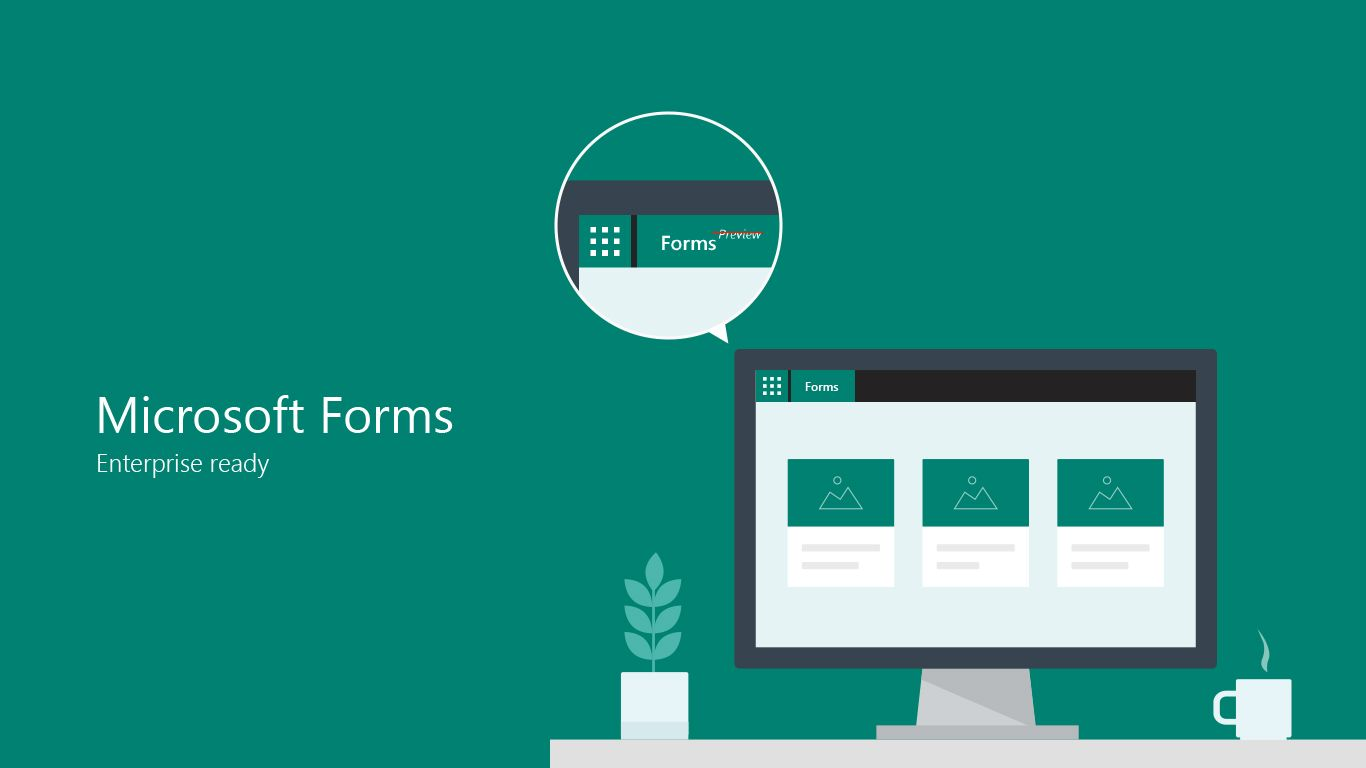
\includegraphics[width=0.3\textwidth]{MicrosoftForms.png}
	\caption{Figuur 4.11 heeft een weergave van Microsoft Forms. }
\end{figure}


 \chapter{\IfLanguageName{dutch}{Resultaten}{Resultaten}}
\label{ch:Resultaten}
In dit hoofdstuk zullen de resultaten van de testen en de enquête verwerkt worden om zo tot een antwoord te komen op dit onderzoek. Hierbij zijn de resultaten van de Cisco Identity Services Engine omgeving opgedeeld in 'Port-based en Policy-based network access control' en 'Tread-Centric en Policy-based network access control'. Vervolgens zijn de enquête resultaten verwerkt met een aantal diagrammen. Deze resultaten zijn ingedeelt per vraag. 

\section{Cisco Identity Services Engine omgeving}
Zoals men ziet wordt Policy-based network access control steeds gecombineerd met Port-based en Thead-Centric network access control. Dit heeft als rede dat voor zowel Port-based, als voor Thread-Centric network access control, policy rules zijn toegepast.


\subsection{Port-based en Policy-based network access control}
Wanneer 'Port-based en Policy-based network access control' niet zijn toegepast. Dan ziet men dat gebruikers zich kunnen aansluiten op het netwerk zonder enige beveiliging. Natuurlijk moeten de poorten ingesteld worden met het correcte vlan id om trafiek toe te laten. Maar het is enerzijds duidelijk dat het aansluiten op het netwerk via de poorten veel eenvoudiger is. 
\newline
\newline
Als men de resultaten van 'Port-based en Policy-based network access control' er bij halen. Dan ziet men een duidelijk verschil in beveiliging  met of zonder de use cases. Wanneer een gebruiker zich wenst aan te melden op het netwerk via een van de poorten op de fysieke Cisco switch. Dan wordt geen trafiek toegelaten op het netwerk. Dit resulteert in het ontvangen van ip adres van de vorm 169.254.x.x, dat geen enkel compartiment van het netwerk kan bereiken.
 
\begin{figure}[H]
	\centering
	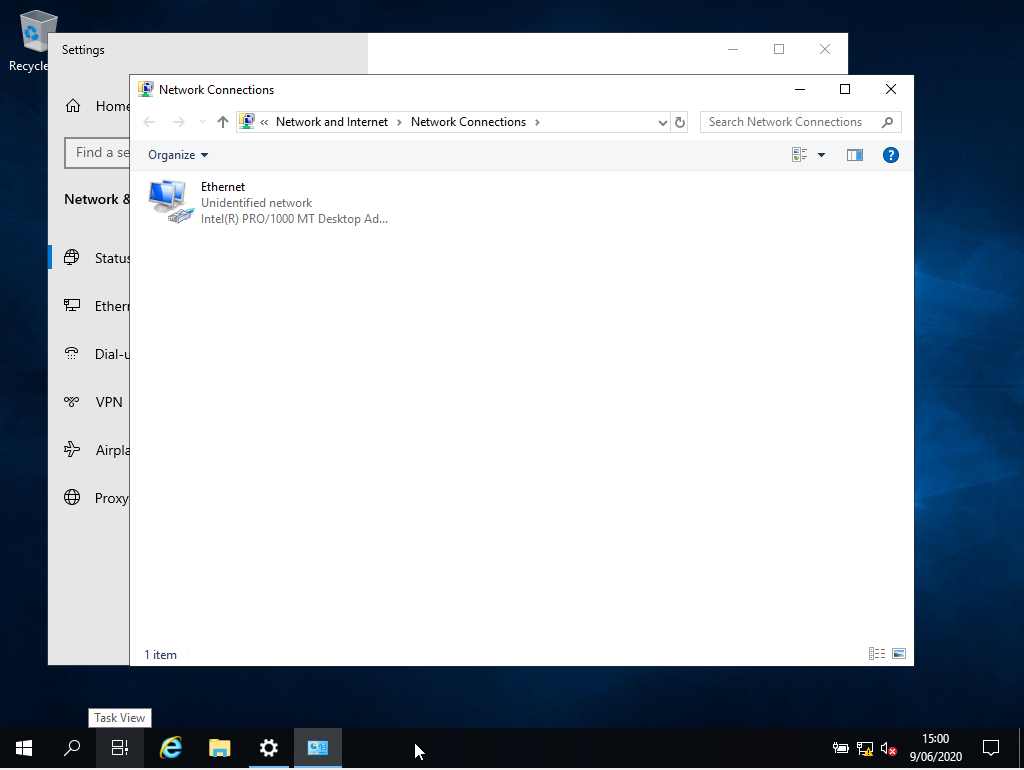
\includegraphics[height=0.40\textheight]{Port_no_network_access.png}
	\caption{Deze afbeelding geeft aan dat het apparaat niet met het netwerk is verbonden, wanneer men aansluit op één van de poorten op de Cisco switch.}
\end{figure}

\begin{figure}[H]
	\centering
	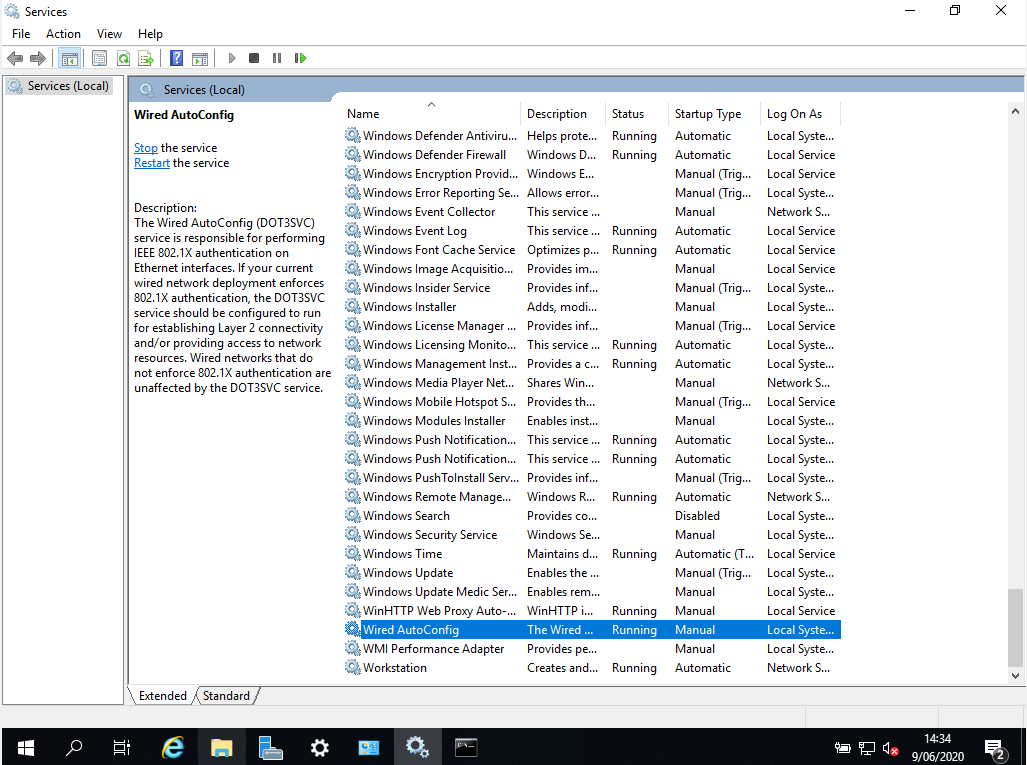
\includegraphics[height=0.40\textheight]{Service_ise_port.png}
	\caption{Deze afbeelding geeft de service 'Wired AutoConfig' weer.}
\end{figure}
\newpage
Het is echter wanneer men de 'Wired AutoConfig' services aanzet, kan men zich aanmelden op het netwerk door volgende stappen uit te voeren: 
\newline

\begin{itemize}
	\item Open het configuratiescherm, en ga naar 'netwerk en internet'.
	\item Open vervolgens het 'netwerkcentrum'.
	\item Open 'Adapter instellingen wijzigen'.
	\item Open het 'properties' tablad, door rechtermuisklik op de  correcte "Ehternet adapter".
	\item Vervolgens ziet men het tablad "Authenticatie".
	\item Open "Extra instellingen".
	\item Veranderd het de 'authentication modus' naar gebruikers authenticatie.
	\newline
\end{itemize}


Het is echter wanneer men het juiste gebruikersnaam en wachtwoord ingeeft, dan wordt de gebruiker met zijn apparaat aangesloten op het netwerk. Vervolgens is ook een policy rule geïmplementeerd dat alleen gebruikers van de groep 'Employees' kunnen aanmelden op het netwerk via één van de Cisco poorten. Dit werd echter al eerder vernoemd in het proof of concept hoofdstuk. 
\newline
\newline
Het is enigszins duidelijk dat wanneer men wenst in te loggen met de gebruiker 'Test' en het wachtwoord 'Admin2020', dat men geen toegang krijgt tot het netwerk. Dit komt omdat gebruiker 'Test' zich niet in de groep 'Employees' bevindt. Hierdoor is aangetoond dat het gebruik van policies ook de vruchten plukt op beveiliging.

\begin{figure}[H]
	\centering
	\subfloat{{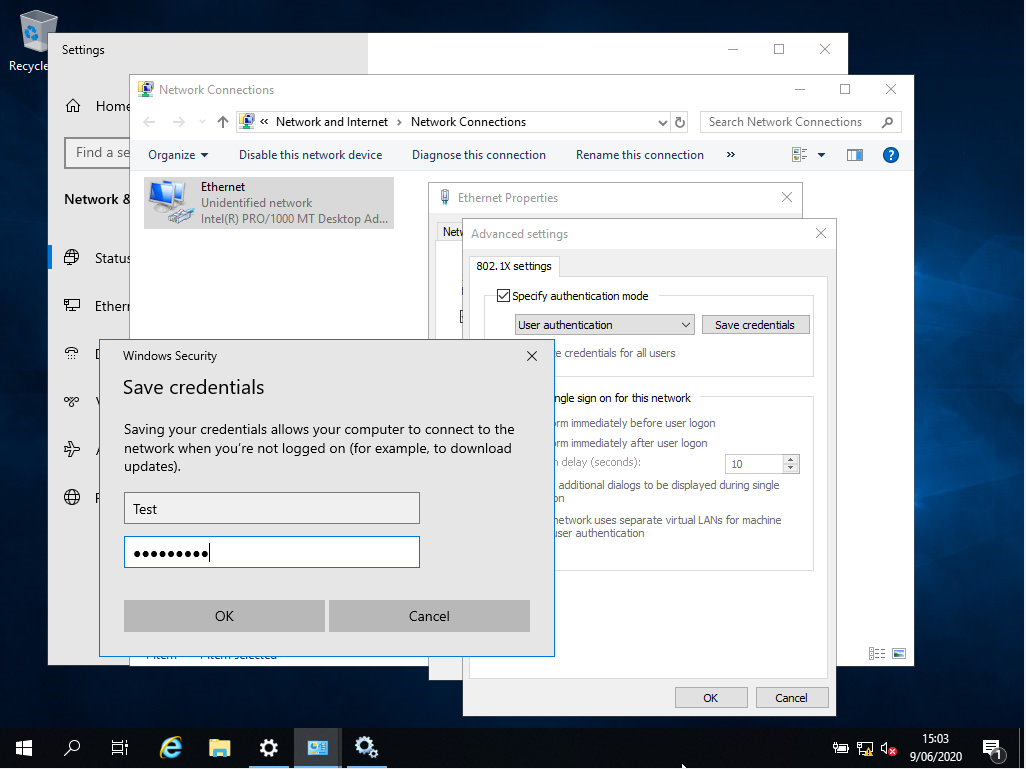
\includegraphics[width=6.5cm]{Test_no_employee.png} }}%
	\qquad
	\subfloat{{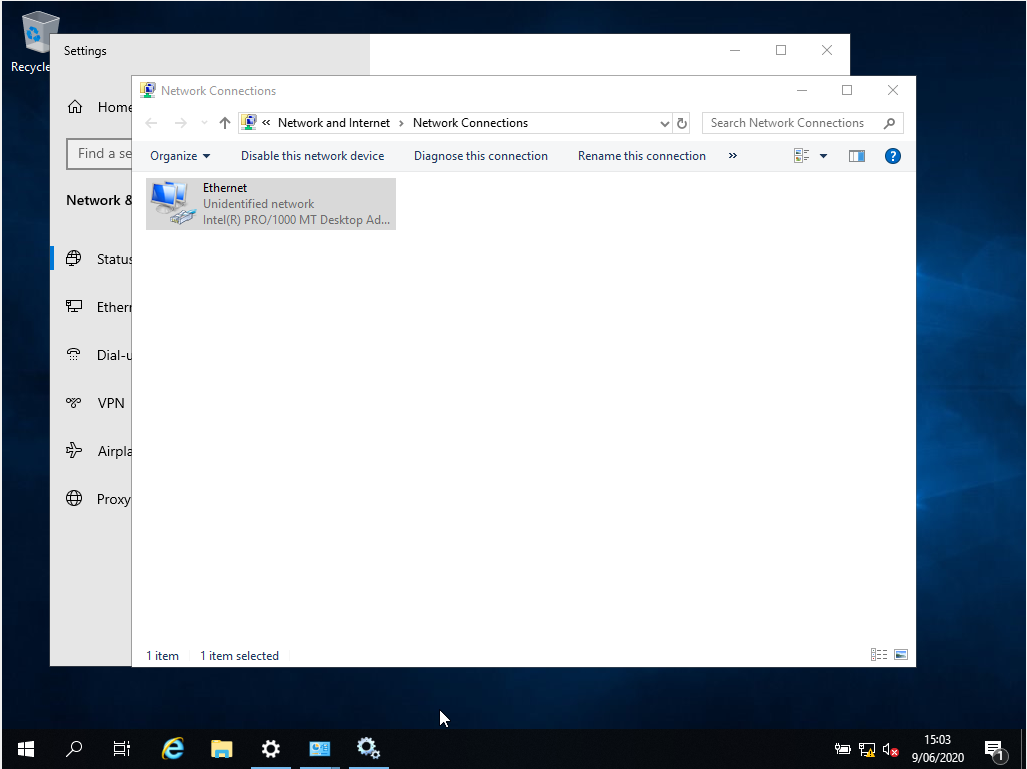
\includegraphics[width=6.5cm]{Test_no_successed.png} }}%
	\newline
	\qquad
	\subfloat{{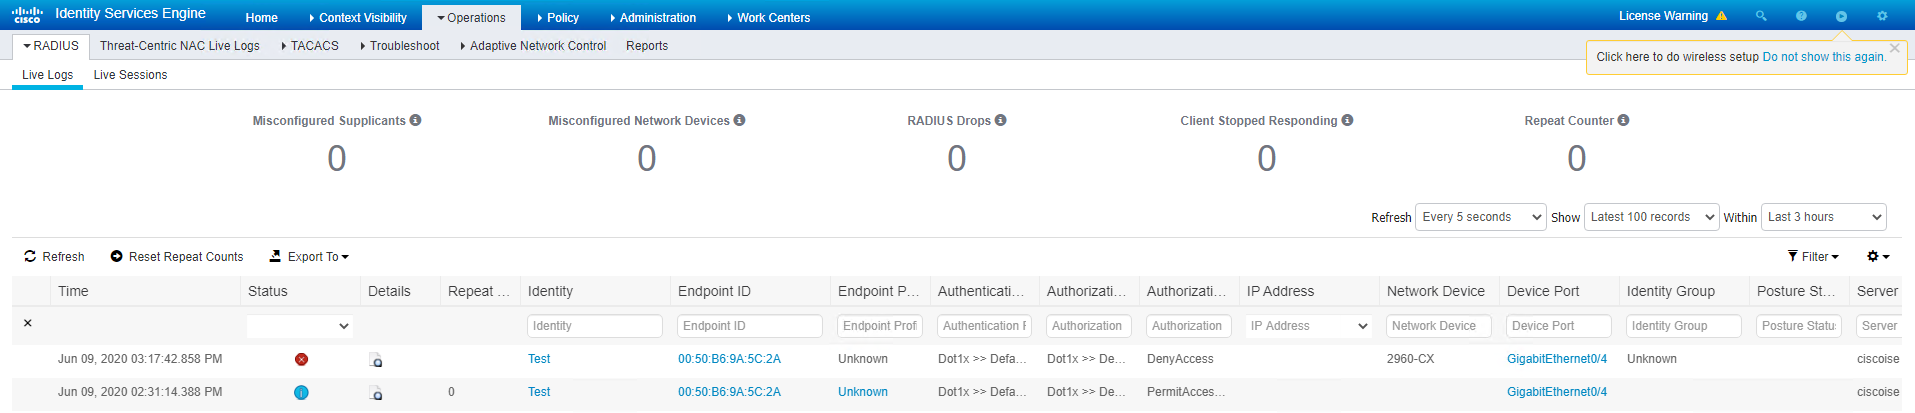
\includegraphics[width=14cm]{TestDenied.png} }}%
	\caption{Bovenstaande foto's geven aan dat gebruiker 'Test' zich niet kan aansluiten op het netwerk. Omdat de gebruiker 'Test' niet in de groep 'Employees' bevindt.}%
	\label{fig:Test_gebruiker}%
\end{figure}
	
Als men wenst in te loggen met een gebruiker die zich in de ISE groep 'Employees' bevindt, dan zal deze gebruiker met zijn apparaat via een poort kunnen aansluiten op het netwerk. 
\newline
\newline
Wanneer de test met gebruiker 'TestV2', die zich in de groep 'Employees' bevindt, uitgevoerd wordt. Dan is het vanzelfsprekend dat deze gebruiker met zijn apparaat met het netwerk kan verbinden.

\begin{figure}[H]
	\centering
	\subfloat{{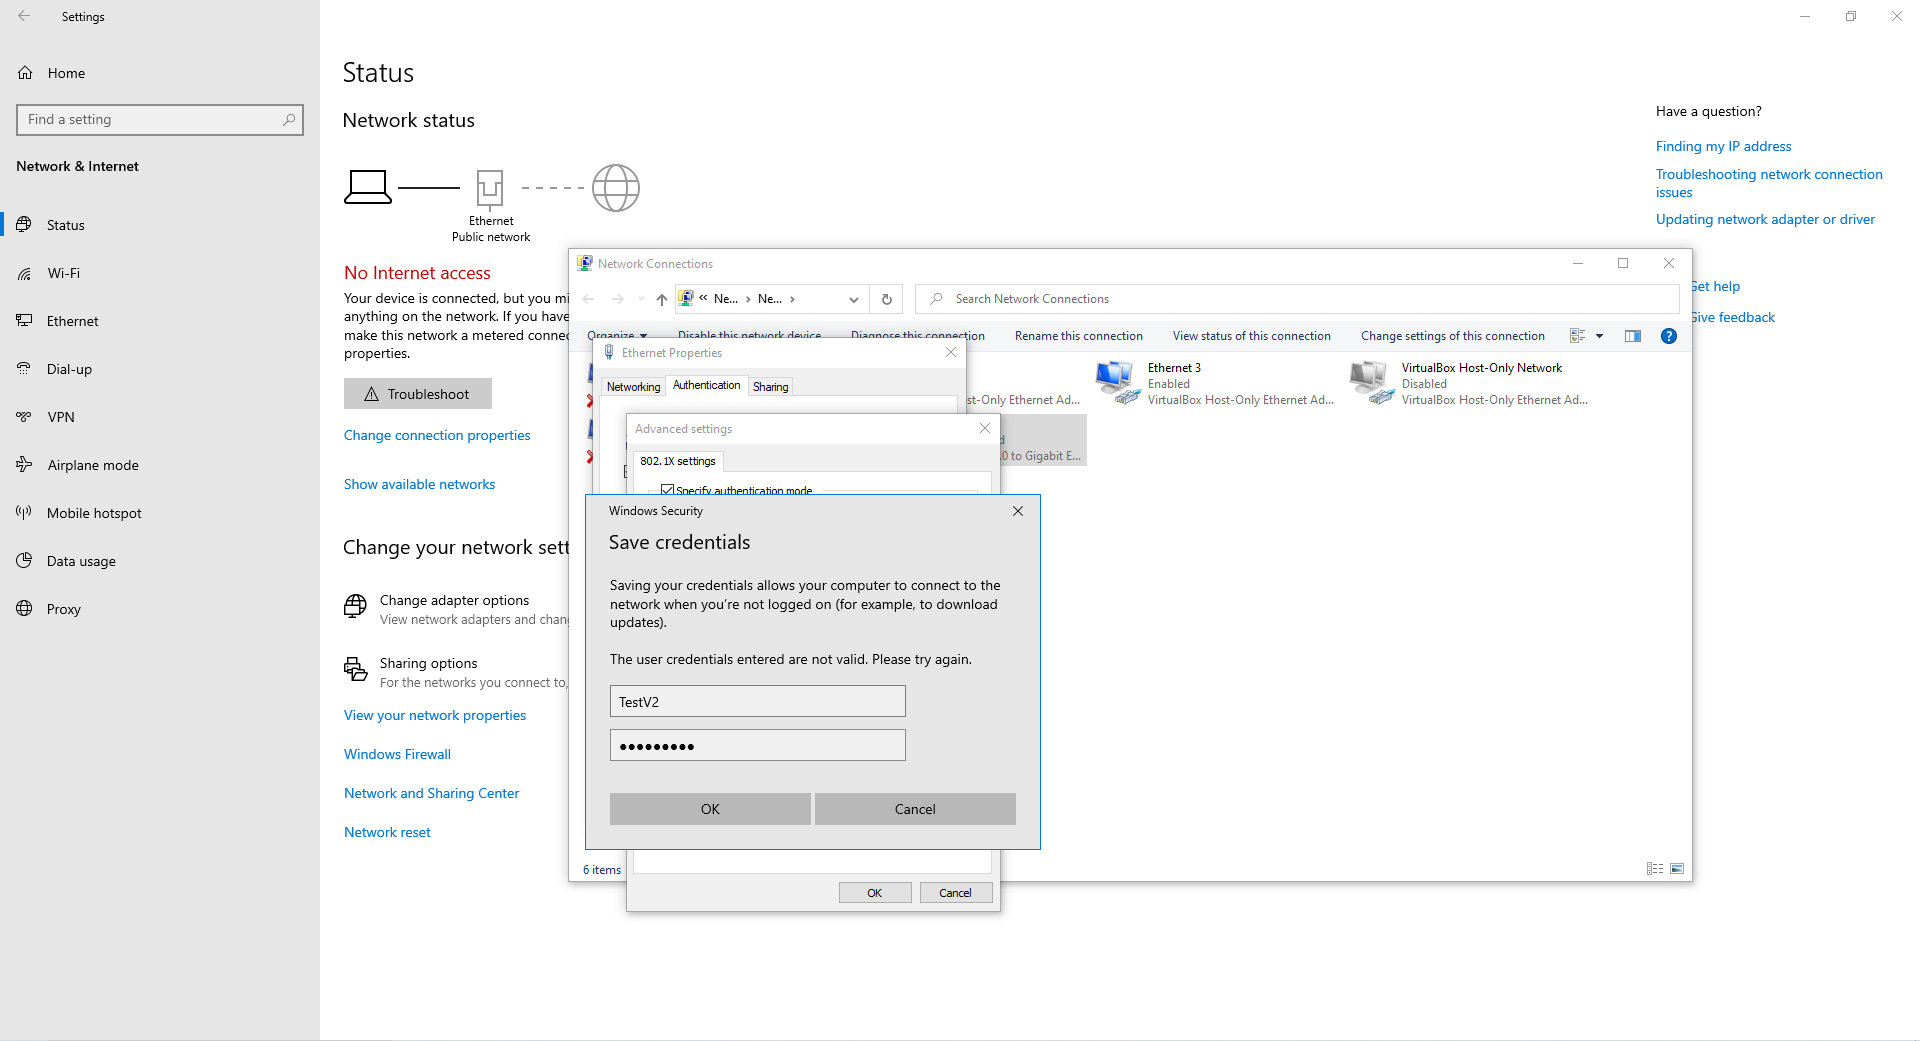
\includegraphics[width=6.5cm]{TestV2_Employee.png} }}%
	\qquad
	\subfloat{{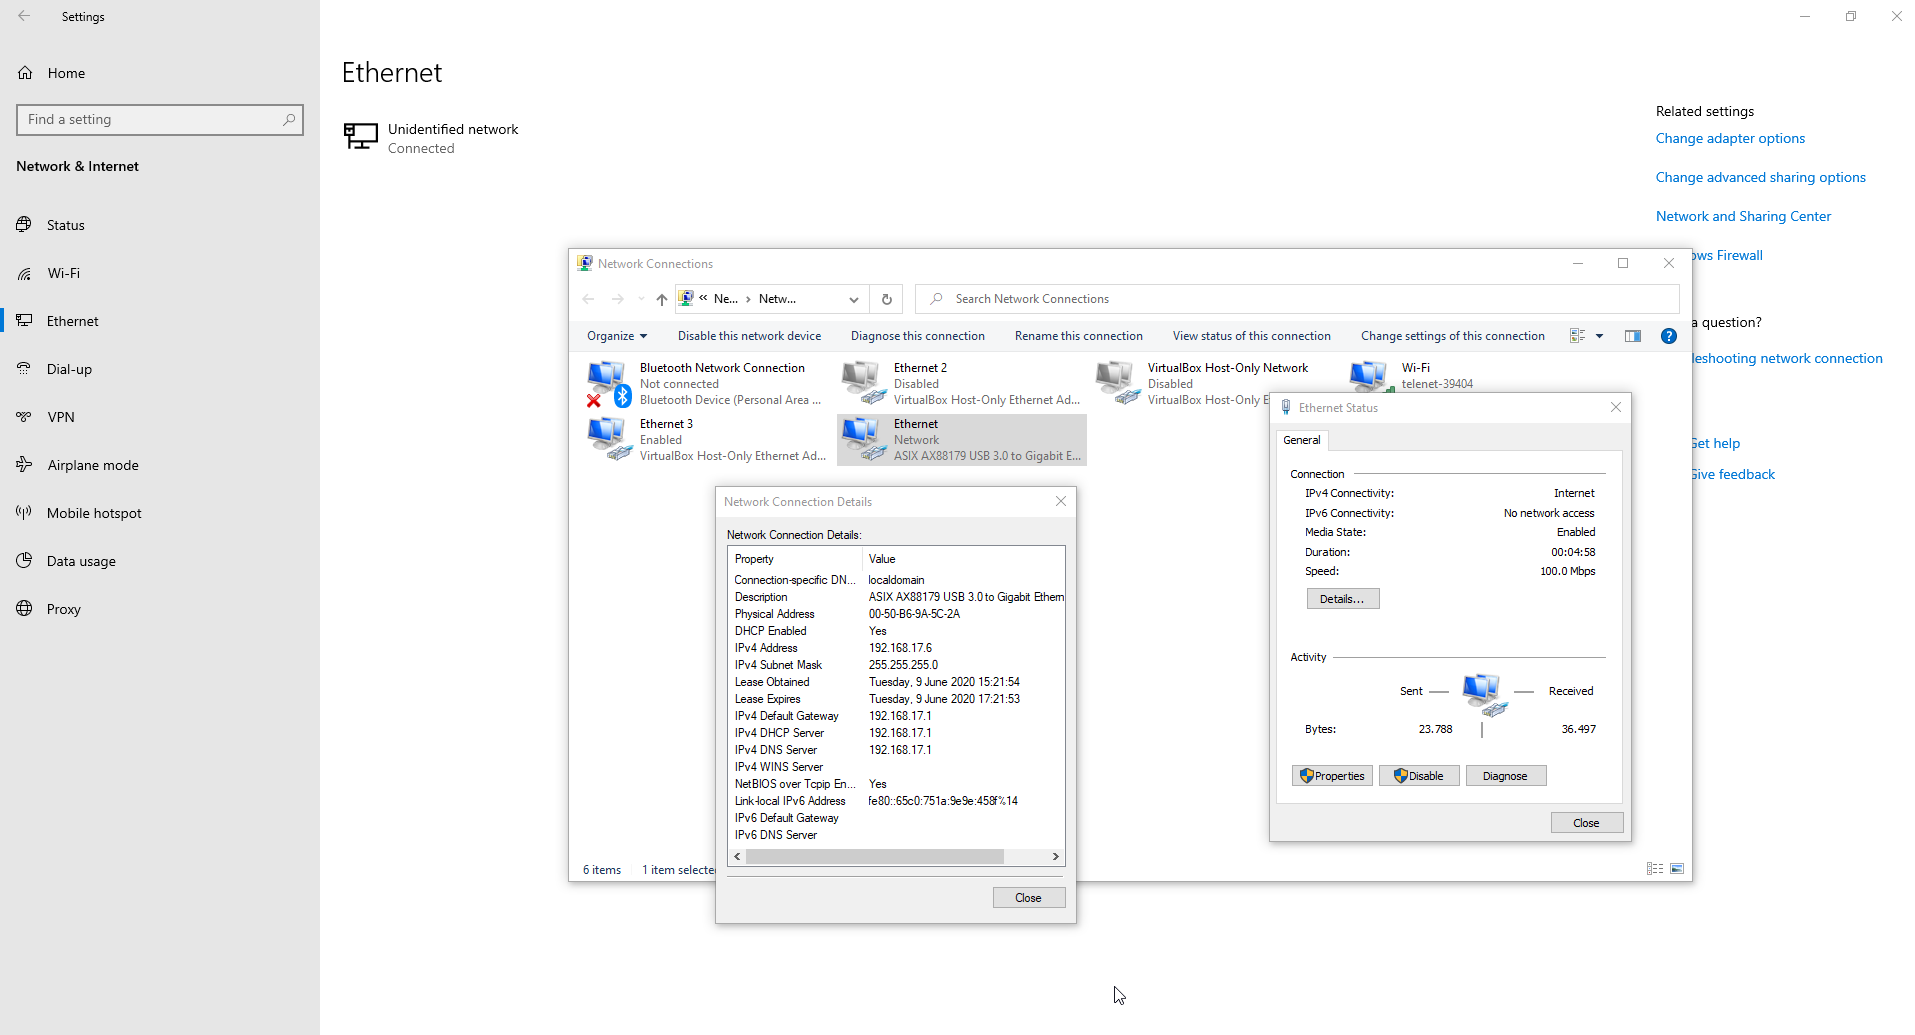
\includegraphics[width=6.5cm]{TestV2_succeeded.png} }}%
	\newline
	\qquad
	\subfloat{{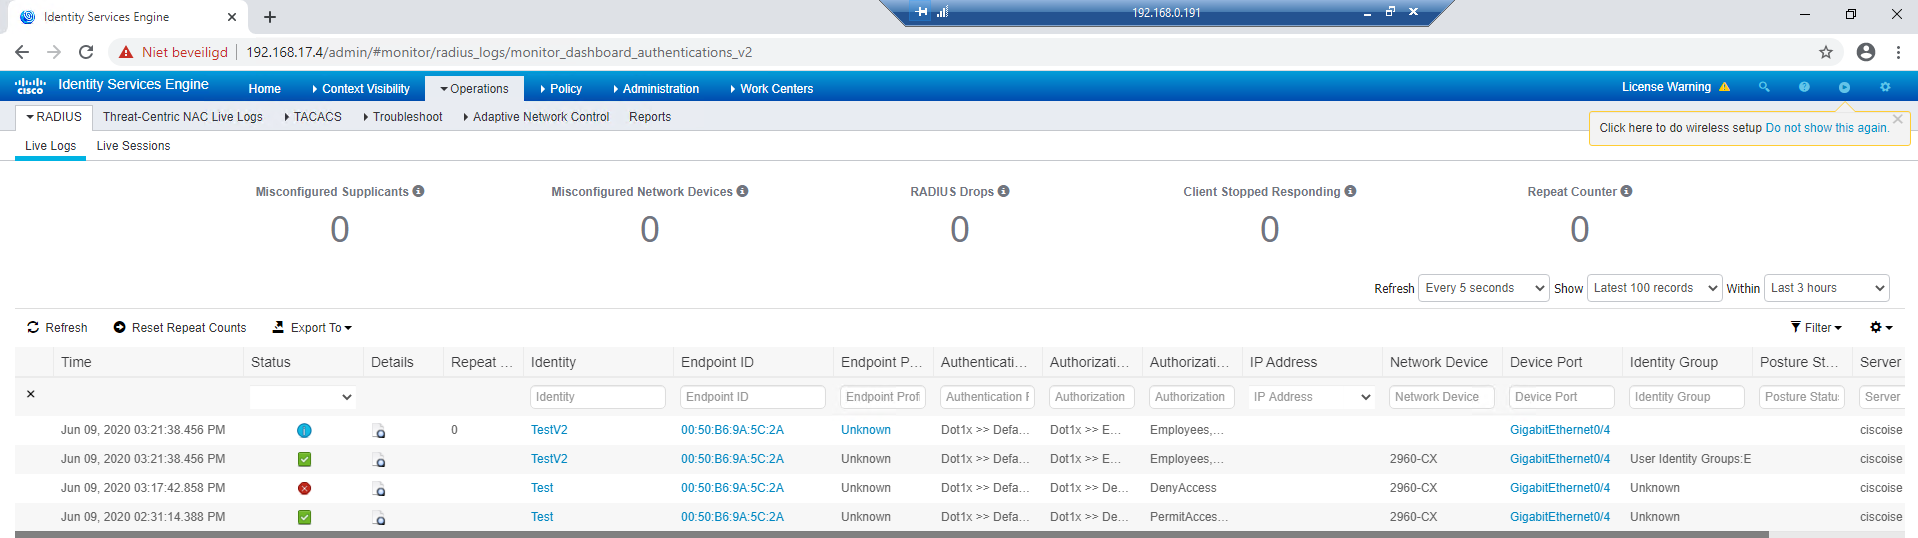
\includegraphics[width=14cm]{TestV2_succeeded_ISE.png} }}%
	\caption{Bovenstaande foto's geven aan dat gebruiker 'TestV2' zich kan aansluiten op het netwerk. Omdat de gebruiker 'TestV2' zich in de groep 'Employees' bevindt.}%
	\label{fig:Test_gebruiker}%
\end{figure}

Hierdoor is aangetoond dat Cisco Idendity Services Engine met use cases 'Port-based en Policy-based network access control' een positieve uitkomst bekomt. M.a.w. plukt 'Port-based en Policy-based network access control' de vruchten af op security vlak. In de volgende subsectie zullen de resultaten van Tread-Centric en Policy-based network access control besproken worden.


\subsection{Tread-Centric en Policy-based network access control}
\section{Cisco Identity Services Engine enquête}

\begin{figure}[H]
	\centering
	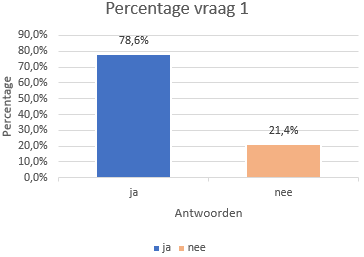
\includegraphics[height=0.30\textheight]{Vraag1.png}
	\caption{Deze afbeelding geeft de service 'Wired AutoConfig' weer.}
\end{figure}

\begin{figure}[H]
	\centering
	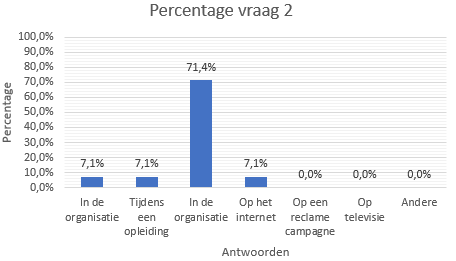
\includegraphics[height=0.30\textheight]{Vraag2.png}
	\caption{Deze afbeelding geeft de service 'Wired AutoConfig' weer.}
\end{figure}

\begin{figure}[H]
	\centering
	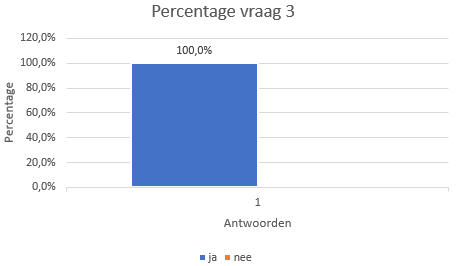
\includegraphics[height=0.40\textheight]{Vraag3.png}
	\caption{Deze afbeelding geeft de service 'Wired AutoConfig' weer.}
\end{figure}

\begin{figure}[H]
	\centering
	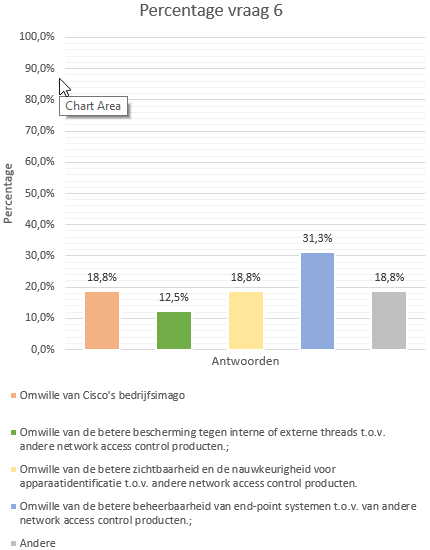
\includegraphics[height=0.30\textheight]{Vraag6.png}
	\caption{Deze afbeelding geeft de service 'Wired AutoConfig' weer.}
\end{figure}

\begin{figure}[H]
	\centering
	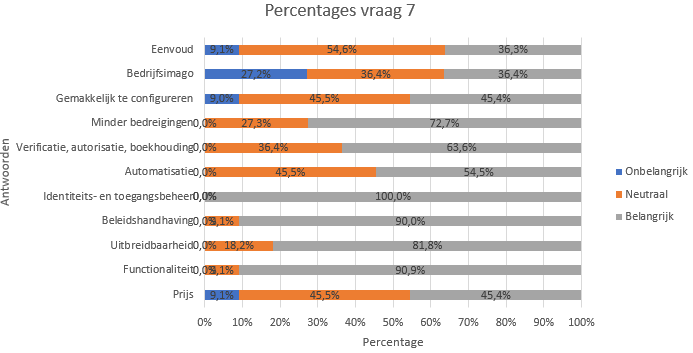
\includegraphics[height=0.30\textheight]{Vraag7.png}
	\caption{Deze afbeelding geeft de service 'Wired AutoConfig' weer.}
\end{figure}

\begin{figure}[H]
	\centering
	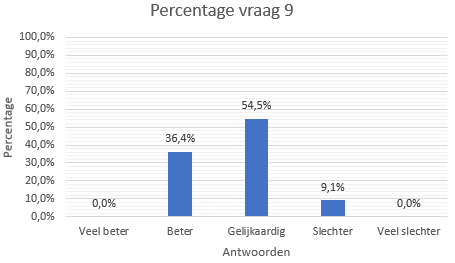
\includegraphics[height=0.30\textheight]{Vraag9.png}
	\caption{Deze afbeelding geeft de service 'Wired AutoConfig' weer.}
\end{figure}

\begin{figure}[H]
	\centering
	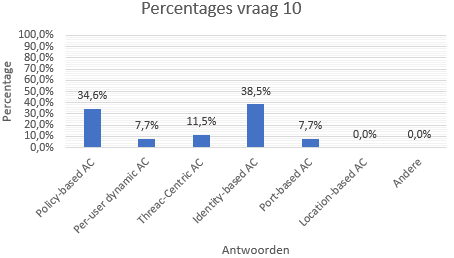
\includegraphics[height=0.30\textheight]{Vraag10.png}
	\caption{Deze afbeelding geeft de service 'Wired AutoConfig' weer.}
\end{figure}

\begin{figure}[H]
	\centering
	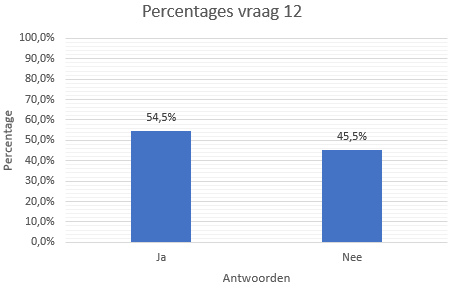
\includegraphics[height=0.30\textheight]{Vraag12.png}
	\caption{Deze afbeelding geeft de service 'Wired AutoConfig' weer.}
\end{figure}
\begin{figure}[H]
	\centering
	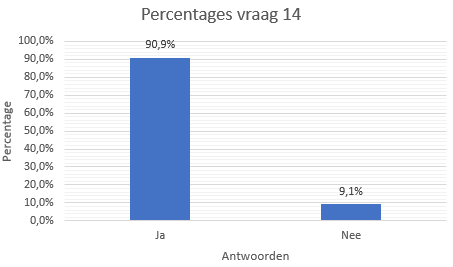
\includegraphics[height=0.30\textheight]{Vraag14.png}
	\caption{Deze afbeelding geeft de service 'Wired AutoConfig' weer.}
\end{figure}
\begin{figure}[H]
	\centering
	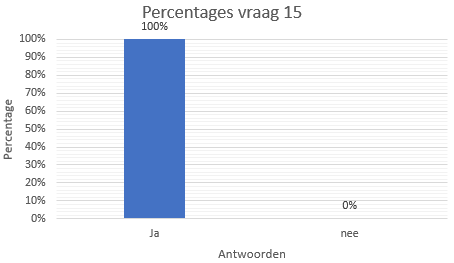
\includegraphics[height=0.30\textheight]{Vraag15.png}
	\caption{Deze afbeelding geeft de service 'Wired AutoConfig' weer.}
\end{figure}
\begin{figure}[H]
	\centering
	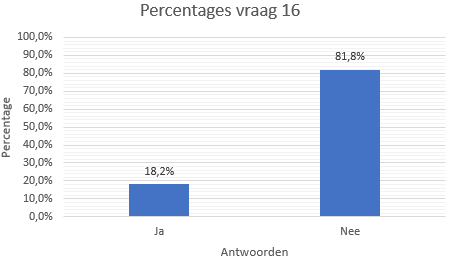
\includegraphics[height=0.30\textheight]{Vraag16.png}
	\caption{Deze afbeelding geeft de service 'Wired AutoConfig' weer.}
\end{figure}
\begin{figure}[H]
	\centering
	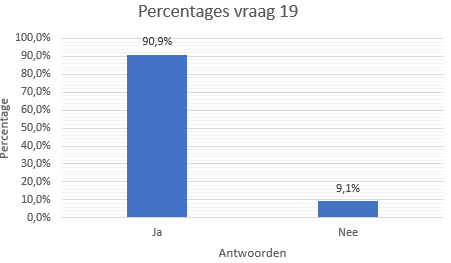
\includegraphics[height=0.30\textheight]{Vraag19.png}
	\caption{Deze afbeelding geeft de service 'Wired AutoConfig' weer.}
\end{figure}
\begin{figure}[H]
	\centering
	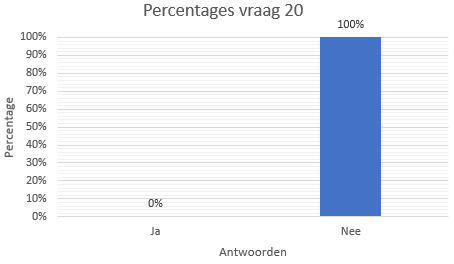
\includegraphics[height=0.30\textheight]{Vraag20.png}
	\caption{Deze afbeelding geeft de service 'Wired AutoConfig' weer.}
\end{figure}



%%=============================================================================
%% Conclusie
%%=============================================================================

\chapter{Conclusie}
\label{ch:conclusie}

% TODO: Trek een duidelijke conclusie, in de vorm van een antwoord op de
% onderzoeksvra(a)g(en). Wat was jouw bijdrage aan het onderzoeksdomein en
% hoe biedt dit meerwaarde aan het vakgebied/doelgroep? 
% Reflecteer kritisch over het resultaat. In Engelse teksten wordt deze sectie
% ``Discussion'' genoemd. Had je deze uitkomst verwacht? Zijn er zaken die nog
% niet duidelijk zijn?
% Heeft het onderzoek geleid tot nieuwe vragen die uitnodigen tot verder 
%onderzoek?

\lipsum[76-80]


'
%%=============================================================================
%% Bijlagen
%%=============================================================================

\appendix
\renewcommand{\chaptername}{Appendix}

%%---------- Onderzoeksvoorstel -----------------------------------------------

\chapter{Onderzoeksvoorstel}

Het onderwerp van deze bachelorproef is gebaseerd op een onderzoeksvoorstel dat vooraf werd beoordeeld door de promotor. Dat voorstel is opgenomen in deze bijlage.

% Verwijzing naar het bestand met de inhoud van het onderzoeksvoorstel
%---------- Inleiding ------------s---------------------------------------------

\section{Introductie} % The \section*{} command stops section numbering
\label{sec:introductie}
Tijdens deze uiteenzetting zal voornamelijk beschreven worden hoe Network Access Control door het gebruik van de technologie Cisco Identity Service Engine (\cite{CiscoISE}) gebruikt wordt.\\Door principes zoals Bring Your Own Device (BYOD) en Internet Of Things (IoT) is er steeds meer vraag naar de bussiness resources van de verschillende endpoint-systemen vanuit het perspectief van de werknemers of de IoT-systemen. Bedrijven moeten de proliferatie netwerk-compatibele apparaten beter ondersteunen, zelfs wanneer een groot aantal cyber bedreigingen en veel gepubliceerde datalekken aantonen dat het belang van bescherming over de toegang tot de ontwikkelende bedrijfsnetwerken van cruciaal belang is.\\Door integratie van Cisco Identity Service Engine kan er een betere bescherming gegarandeerd worden tegen deze exponentiële toename van geconnecteerde systemen. Kortom kan het netwerk veiliger en meer beheerbaar gemaakt worden. Uit deze informatie kan een antwoord op de volgende onderzoeksvragen een oplossing bieden in dit probleemveld. De onderzoeksvragen luiden als volgt: Hoe kunnen we een evoluerend bedrijfsnetwerk beter beheren en beveiligen door het gebruik van Cisco Identity Service Engine? Hoe zorgen we voor een veiliger IT netwerk met principes zoals Internet Of Things en Bring Your Own Device? Wat zijn de positieve en negatieve gevolgen door het gebruik van Cisco Identity Service Engine?\\ \\Cisco Identity Service Engine is een groot platform waar vele uitbreidingen en use cases mogelijk zijn, daarom zal Policy Based Access Control, Threat-centric Network Access Control en Port-based Network Access Control als basis toegepast worden tijdens de uiteenzetting van deze bachelorproef.

%---------- Stand van zaken ---------------------------------------------------
\pagebreak
\section{Literatuurstudie}
\label{sec:Literatuurstudie}
U vraagt zich waarschijnlijk af wat termen zoals Network Access Control, Policy Based Access Control, Threat-centric Network Access Control en Port Based Network Access Control nu eigenlijk betekenen?\\Volgens \cite{Cisco} is Network Access Control, een oplossingen die netwerkzichtbaarheid en toegangsbeheer ondersteunt door middel van beleidshandhaving op apparaten en gebruikers in bedrijfsnetwerken. Organisaties moeten rekening houden met de veiligheidsrisico's van de exponentiële groei van verscheidene endpoint-systemen die toegang hebben op het bedrijfsnetwerk. Cisco beweert dat het van cruciaal belang is om over de correcte tools te beschikken die het netwerkbeveiligings infrastructuur versterken.

\subsection{Network Access Control use cases}
Zaken zoals Policy Based Access Control, Threat-centric Network Access Control en Port Based Network Access Control zijn termen die gezien worden als use cases of als uitbreiding van de Network Access Control technologie. Deze use cases hebben allemaal als functie het netwerk veilig te maken tegen interne of externe threads. Zo zorgt volgens \cite{jerichosystems.net} Policy Based Access Control voor een beter digitaal beheer dat bestaat uit verschillende regels om beslissingen te nemen op de authorization levels. \\\cite{TC-NAC} citeert dat Threat-centric Network Access Control zich ontfermt over het creëren van policies die gebaseerd zijn 
op de bedreigings- en kwetsbaarheidskenmerken die komen vanuit endpoint systemen. Als laatste term hebben we Port Based Network Access Control,\\\cite{juniper.net} vertelt ons dat Port Based Network Access Control, Ethernet-interfaces valideert om ongeautoriseerde toegang tot een opgegeven routerpoort te voorkomen. Voordat deze authenticatie voltooid is, zijn alleen de 802.1x-besturingspakketten toegestaan en worden deze doorgestuurd naar de router voor verwerking. De overige besturingspakketten worden verwijderd.


\subsection{Award uitreiking}
De award uitreiking die Frost and Sullivan heeft uitgevoerd over Cisco Identity Service Engine wordt tijdens deze sectie aangehaald. Gebaseerd op recente analyses en onderzoeken van wereldwijde Network Access Controls, erkent \cite{Frost&Sullivan} Cisco Systems met de Global Market Leadership Award voor het veroveren van ongeveer 35 percent van de markt. Dit heeft vooral te maken met Cisco's brede portfolio van beveiligingsproducten. Volgens Frost en Sullivan heeft Cisco Identity Services Engine de grote bedrijfssegmenten volledig gedomineerd. De integratie van Cisco Identity Service Engine brengt veel uitgebreide en schaalbare oplossingen met zich mee, die een breed gamma aan functies hebben. \\ \\ Cisco won de uitreiking van de Global Market Leadership Award mede dankzij de recente release van de Identity Service Engine 2.4. De release van 2.4 breidt zijn talrijke functies uit naar opkomende industriële markten, zoals Internet of Things, de industrie- en de gezondheidszorgmarkt. Cisco werkt hiervoor samen met ziekenhuizen, fabrieken, etc.. , om een oplossing te ontwikkelen die niet enkel medische systemen identificeert, maar ook helpt bij het definiëren van het toegangsniveau's van systemen op het netwerk.
%--Hier beschrijf je de \emph{state-of-the-art} rondom je gekozen onderzoeksdomein. Dit kan bijvoorbeeld een literatuurstudie zijn. Je mag de titel van deze sectie ook %--aanpassen (literatuurstudie, stand van zaken, enz.). Zijn er al gelijkaardige onderzoeken gevoerd? Wat concluderen ze? Wat is het verschil met jouw onderzoek? Wat %--is de relevantie met jouw onderzoek?

%--Verwijs bij elke introductie van een term of bewering over het domein naar de vakliteratuur, bijvoorbeeld~\autocite{Doll1954}! Denk zeker goed na welke werken je %--refereert en waarom.

% Voor literatuurverwijzingen zijn er twee belangrijke commando's:
% \autocite{KEY} => (Auteur, jaartal) Gebruik dit als de naam van de auteur
%   geen onderdeel is van de zin.
% \textcite{KEY} => Auteur (jaartal)  Gebruik dit als de auteursnaam wel een
%   functie heeft in de zin (bv. ``Uit onderzoek door Doll & Hill (1954) bleek
%   ...'')

%--Je mag gerust gebruik maken van subsecties in dit onderdeel.

%---------- Methodologie ------------------------------------------------------
\section{Methodologie}
\label{sec:methodologie}
Om het onderzoek tot een goed einde te brengen, zullen onderzoekstechnieken zoals experimenten, simulaties, implementatie en eventuele enquêtes worden toegepast tijdens dit onderzoek. Axians zal hiervoor een testomgeving voorzien waar Cisco Identity Service Engine uitgerold kan worden. Deze uitvoering zal samen met Policy Based Access Control en threat-Centric Network Access Control geïmplementeerd worden. Indien de tijd dit toelaat, is er een mogelijkheid om extra Use cases te gaan implementeren in de testomgeving om het onderzoek naar een beter beheerbaar en veiliger groeiend bedrijfsnetwerk uit te breiden. Daarnaast zullen er een aantal experimenten en simulaties uitgevoerd worden. Dit laat het toe om acties van uit de werkelijkheid na te bootsen in de voorziene testomgeving. Een mogelijk voorbeeld van experiment kan zijn dat men door de integratie van Threat-Centric Network Access Control het mogelijk maakt dat een geïnfecteerd endpoint-systeem automatisch "weg geknipt" 
wordt uit het bedrijfsnetwerk. Deze actie voorkomt dus dat andere endpoint-systemen ook geïnfecteert zullen raken.\\ \\Om het onderzoek verder aan te vullen, kunnen er enquêtes worden opgesteld. Op deze manier kan in kaart gebracht worden waarom, Axians Cisco Identity Service Engine verkiest boven een andere NAC technologie, welke positieve en negatieve punten Axians ondervindt bij het gebruik van Cisco Identity Service Engine, of indien Axians een daling van interne of externe threads ondervindt sinds de implementatie van Cisco Identity Service Engine.
%--Hier beschrijf je hoe je van plan bent het onderzoek te voeren. Welke onderzoekstechniek ga je toepassen om elk van je onderzoeksvragen te beantwoorden? Gebruik je %--hiervoor experimenten, vragenlijsten, simulaties? Je beschrijft ook al welke tools je denkt hiervoor te gebruiken of te ontwikkelen.


%---------- Verwachte resultaten ----------------------------------------------
\section{Verwachte resultaten}
\label{sec:verwachte_resultaten}
%De bedoeling van deze sectie is om de verwachten resultaten op te stellen over een aantal variabelen die we wensen te testen.
De bedoeling van deze sectie is om stil te staan over de verwachte resultaten van het onderzoek. Op het einde van het onderzoek moet het belang van een Network Access Control aangetoond worden. Eveneens wordt een zeer snelle handeling verwacht tijdens een ramp scenario door het gebruik van Threat-Centric Network Access Control. Dit kan aangetoond worden door het uitvoeren van talrijke experimenten die acties uit de werkelijkheid nabootsen. Daarom wordt de nadruk zeer hard gelegd op een zo goed mogelijke implementatie. Enkel op deze manier kan er aangetoond worden dat de implementatie hierbij leidt tot een veiliger, beheerbaar netwerk. Er wordt verwacht dat de kans op succesvolle cyberaanvallen door de interne en externe threads aanzienlijk kleiner zal zijn door het gebruik van Cisco Identity Service Engine. Dit kunnen we perfect aantonen door gebruik te maken van een mockgrafiek. Door het gebruik van mockgrafieken wordt er een beter visueel beeld gecreëerd van de resultaten.
%\begin{wrapfigure}{2}{0.15\textwidth}
%	\centering
%	\includegraphics[height=0.55\textwidth,height=.35\textheight]{images/KansRampSenarios.jpg}
%\end{wrapfigure}
\\ \\
\begin{figure}[!t]
	\centering
	\textbf{Kans op succesvolle cyberaanvallen}\par\medskip
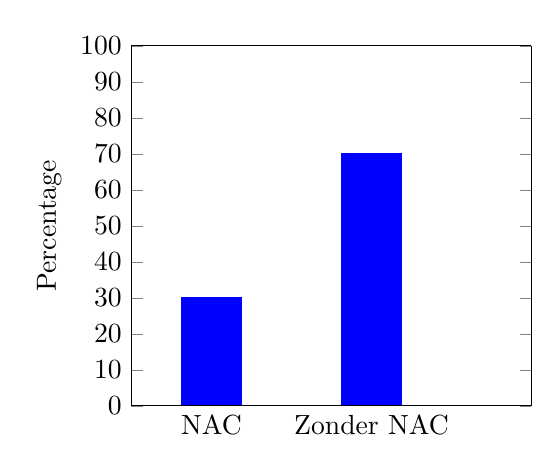
\begin{tikzpicture}
\begin{axis}[
	/pgf/number format/1000 sep={},
	width=2.0in,
	height=1.8in,
	at={(0.758in,3in)},
	scale only axis,
	clip=false,
	separate axis lines,
	axis on top,
	xmin=0,
	xmax=5,
	xtick={1,2,3},
	x tick style={draw=none},
	xticklabels={NAC, ,Zonder NAC},
	ytick={0,10,20,30,40,50,60,70,80,90,100},
	ymin=0,
	ymax=100,
	ylabel={Percentage},
	every axis plot/.append style={
		ybar,
		bar width=0.3in,
		bar shift=0pt,
		fill
	}
	]
	\addplot[blue]coordinates{(1,30)};
	\addplot[blue]coordinates{(3,70)};
\end{axis}
\end{tikzpicture}
\end{figure}

%---------- Verwachte conclusies ----------------------------------------------
\section{Verwachte conclusies}
\label{sec:verwachte_conclusies}
Wanneer de resultaten van het onderzoek aanduiden dat bedrijven die NAC technologieën implementeren, hun endpoint systemen beter kunnen beheren en beveiligen tegen interne en externe threads. Dan kunnen we concluderen dat het belang van deze implementaties rondom de Network Access Control technologieën een belangrijke must is. Daarnaast verwachten we ook dat het percentage op cyberaanvallen op het netwerk aanzienlijk kleiner zal zijn. Bovendien verwachten we dat met het gebruik van Network Access Control in combinatie met Threat-centric Network Access Control een zeer snelle handeling gebeurt wannneer endpoint systemen virussen of malware bevat.

%--Hier beschrijf je wat je verwacht uit je onderzoek, met de motivatie waarom. Het is \textbf{niet} erg indien uit je onderzoek andere resultaten en conclusies vloeien dan dat je hier beschrijft: het is dan juist interessant om te onderzoeken waarom jouw hypothesen niet overeenkomen met de resultaten.



%%---------- Andere bijlagen --------------------------------------------------
% TODO: Voeg hier eventuele andere bijlagen toe
\input{Resultaten enquête}

%%---------- Referentielijst --------------------------------------------------

\printbibliography[heading=bibintoc]

\end{document}
